\input{headers/pacotes}
\input{headers/comandos}

% Dados Gerais
\autor{André Guedes, Caio Nardelli, Jonathan Moraes \\ Matheus Herlan, Matheus Oliveira e Pedro Tomioka}
\curso{Requisitos de Software - 201308 \\ Modelagem de Processos - 203921}

% Dados do trabalho
\titulo{Relatório 02 do Projeto de Melhoria CHAMEX}
\data{04 de Dezembro de 2014}

% Dados da orientacao
\orientador{George Marsicano Corrêa, MSc.}
\coorientador{}

\local{Brasília, DF}
\instituicao{
  Universidade de Brasília - UnB
  \par
  Faculdade UnB Gama - FGA
}
\tipotrabalho{Relatório de Engenharia de Software}
\preambulo{Trabalho submetido durante o curso de graduação em Engenharia de Software da Universidade de Brasília como requisito parcial para obtenção curricular da disciplina de Requisitos de \emph{Software} e Modelagem de Processos.}

\input{headers/setup}

\begin{document}

	\frontmatter
		\frenchspacing
		\imprimircapa
		\renewcommand{\imprimirorientadorRotulo}{ Orientador: }
		\imprimirfolhaderosto
		
		\input{headers/indiceAutomatico}
		\input{headers/listasAutomaticas}
		\begin{siglas}
	\item[Migue] X
\end{siglas}


	\textual

	\mainmatter
	%[RS]	Apresentar o entendimento do contexto de negócio (processo de negócio), no qual os requisitos serão identificados;
		\chapter[Contexto de Negócio]{Contexto de Negócio}
\label{chap:contexto}
	O grupo da disciplina de Requisitos de \emph{Software} (RS) ficou responsável por trabalhar, juntamente com o grupo da disciplina de Modelagem de Processos (MPR), soluções de \emph{software} para o contexto da empresa fictícia CHAMEX.
\\ \indent O objetivo da CHAMEX consiste em auxiliar pequenas e médias empresas privadas a melhorarem a qualidade de vida dos trabalhadores. Quanto mais disposição, vitalidade e alegria obtiver entre os trabalhadores, mais resultado positivo as empresas possuem.
\\ \indent Para concretização do suporte às empresas, a CHAMEX elaborou o Modelo de Avaliação (MOA). O principal objetivo desse modelo está atrelado à verificação do nível de satisfação e qualidade de vida dos funcionários de uma determinada organização. A CHAMEX apresenta um modelo de gestão por processos, tendo em vista que não há divisões de departamentos e caracterização hierárquica interna.
\\ \indent O grupo de MPR realizou um levantamento dos processos existentes dentro da CHAMEX e foram identificados:
\begin{itemize}
	\item{Inscrição no MOA;}
	\item{Seleção dos Avaliadores;}
	\item{Avaliação das Empresas;}
	\item{Validação dos Questionários;}
	\item{Compilação dos Resultados.}
\end{itemize}
\ \indent Dessa maneira, foi necessário avaliar qual dos processos descritos anteriormente seria adotado para melhoria. Assim, o grupo de MPR adotou os seguintes critérios:
\begin{itemize}
	\item{Grau de vinculação com os objetivos organizacionais ou com o direcionamento estratégico da organização;}
	\item{Impacto no cliente externo;}
	\item{Potencial para obtenção de benefícios financeiros ou redução de custos para organização;}
	\item{Impacto na imagem externa.}
\end{itemize}
\ \indent Adicionalmente, foi necessário levar em consideração a viabilidade de melhoria de cada processo. Após consideração destes fatores, o grupo de MPR chegou a conclusão de que o processo de Inscrição no MOA seria o mais apropriado para inserção de melhorias, uma vez que os outros processos apresentaram um valor de viabilidade elevado, caracterizando uma implementação complexa. O processo de Inscrição no MOA apresentou um peso significativo e um valor de viabilidade razoável.

	\section[Identificação e Descrição do Problema]{Identificação e Descrição do Problema}
	\label{sec:contexto_problema}
		Embora o processo escolhido para inserção de melhorias tenha sido a Inscrição no MOA, são apresentados, a seguir, quadros que resumem os problemas encontrados para todo o processo do MOA. É importante ressaltar que os quadros foram construídos com base nas discussões realizadas entre as equipes das disciplinas MPR e RS.

\subsection[Quadros Resumos da Descrição do Problema]{Quadros Resumos da Descrição do Problema}
\label{subsec:contexto_problema_quadros}
	\begin{table}[H]
	\centering
	\begin{tabular}{|p{6cm}|p{9cm}|}
	\hline
	O problema & Empecilhos no atendimento à demanda de solicitação de participação no MOA \\ \hline
	Afeta & Empresa CHAMEX \\ \hline
	O impacto desse problema é & As empresas que desejam participar do MOA não obtêm êxito na solicitação, inviabilizando a participação das mesmas \\ \hline
	Uma solução ideal permitiria & Informatização do processo de análise de solicitação \\ \hline
	\end{tabular}
	\label{tab:problemaUm}
	\caption[Descrição do Problema (1)]{Descrição do Problema (1).}
\end{table}
\begin{table}[H]
	\centering
	\begin{tabular}{|p{6cm}|p{9cm}|}
	\hline
	O problema & Ausência de percepção por parte da CHAMEX do processo do MOA em aplicação nas empresas \\ \hline
	Afeta & Empresa CHAMEX \\ \hline
	O impacto desse problema é & A CHAMEX não possui controle ou percepção total do que está acontecendo nas empresas durante a avaliação \\ \hline
	Uma solução ideal permitiria & Melhorias no relato do status de avaliação de cada empresa \\ \hline
	\end{tabular}
	\label{tab:problemaDois}
	\caption[Descrição do Problema (2)]{Descrição do Problema (2).}
\end{table}
\begin{table}[H]
	\centering
	\begin{tabular}{|p{6cm}|p{9cm}|}
	\hline
	O problema & Os funcionários da CHAMEX devem se locomover para as empresas participantes a fim de aplicar o MOA \\ \hline
	Afeta & Avaliadores e Empresa CHAMEX \\ \hline
	O impacto desse problema é & Os avaliadores ficam fixos em somente um contexo, não havendo flexibilidade \\ \hline
	Uma solução ideal permitiria & Interação entre avaliadores e empresas participantes pela \emph{web} \\ \hline
	\end{tabular}
	\label{tab:problemaTres}
	\caption[Descrição do Problema (3)]{Descrição do Problema (3).}
\end{table}
\begin{table}[H]
	\centering
	\begin{tabular}{|p{6cm}|p{9cm}|}
	\hline
	O problema & Os avaliadores aguardam por longos períodos de tempo o preenchimento dos questionários \\ \hline
	Afeta & Avaliadores \\ \hline
	O impacto desse problema é & Queda de produtividade para os avaliadores, visto que o tempo poderia estar sendo melhor aproveitado para realização de outras atividades \\ \hline
	Uma solução ideal permitiria & Paralelismo e sincronização de tarefas \\ \hline
	\end{tabular}
	\label{tab:problemaQuatro}
	\caption[Descrição do Problema (4)]{Descrição do Problema (4).}
\end{table}
\begin{table}[H]
	\centering
	\begin{tabular}{|p{6cm}|p{9cm}|}
	\hline
	O problema & As empresas participantes não conseguem acompanhar o status da avaliação \\ \hline
	Afeta & Empresas participantes do MOA \\ \hline
	O impacto desse problema é & Em um determinado momento, a empresa participante do MOA não consegue obter uma percepção do status de sua avaliação \\ \hline
	Uma solução ideal permitiria & Acesso imediato ao monitoramento do status da avaliação por parte da Chamex \\ \hline
	\end{tabular}
	\label{tab:problemaCinco}
	\caption[Descrição do Problema (5)]{Descrição do Problema (5).}
\end{table}

\subsection[Diagrama de \emph{Fishbone}]{Diagrama de \emph{Fishbone}}
	\label{subsec:contexto_problema_fishbone}
		Com base nos problemas identificados no processo do MOA, foi construído um Diagrama de \emph{Fishbone}, conforme descrito na Figura \ref{fig:fishbone}, de maneira a possibilitar uma boa percepção do problema principal e das causas raízes.
\begin{landscape}
	\vspace*{\fill}
	\begin{figure}[H]
		\centering
		\includegraphics[scale=0.55]{fishbone}
		\caption[Diagrama de Fishbone]{Diagrama de Fishbone.}
		\label{fig:fishbone}
	\end{figure}
	\vspace*{\fill}
\end{landscape}

	\section[Processo a ser Melhorado]{Processo a ser Melhorado}
	\label{sec:contexto_problema}
		Anteriormente, no primeiro relatório do grupo de MPR, foi definido que o processo priorizado seria o processo de inscrição no MOA. A seguir será apresentada um breve resumo desse processo com o objetivo de contextualizar essa parte do projeto.

\subsection[Inscrição no MOA]{Inscrição no MOA}
\label{subsec:contexto_processoMelhorar_inscricaoMOA}
	\begin{itemize}
	\item{\textbf{Definição}: Permitir que empresas envolvidas no contexto adotado pelo MOA possam solicitar participação e consequentemente serem inscritas, caso sejam autorizadas;}
	\item{\textbf{Responsável}: CHAMEX;}
	\item{\textbf{Outros Participantes}: Empresa que deseja solicitar participação;}
	\item{\textbf{Atividades identificadas no AS-IS}:
		\begin{itemize}
			\item{\textbf{Definir Agenda do MOA}: Criar uma agenda com datas a serem cumpridas;}
			\item{\textbf{Disponibilizar Edital de Participação do MOA}: Disponibilizar edital com informações sobre o MOA;}
			\item{\textbf{Preencher Participação de Solicitação MOA}: Preencher solicitação disponibilizada pela Chamex para que seja possível participar do MOA;}
			\item{\textbf{Avaliação das Solicitações}: Identificar possíveis erros nas solicitações preenchidas pelas empresas como dados inconsistentes ou que estejam faltando;}
			\item{\textbf{Enviar Mensagem de Erro de Preenchimento}: Informar à empresa via e-mail participante quais os erros contidos no preenchimento da solicitação feita por ela;}
			\item{\textbf{Receber Mensagem de Erro de Preenchimento}: Receber via e-mail sobre os erros identificados no preenchimento da solicitação de participação no MOA;}
			\item{\textbf{Analisar Viabilidade de Participação}: Analisar se a empresa que solicitou participação no MOA está contida no contexto elaborado pela Chamex e consequentemente se ela poderá participar do MOA;}
			\item{\textbf{Enviar Resposta para a Empresa}: Informar à empresa via e-mail se ela foi autorizada a participar do MOA;}
			\item{\textbf{Receber Resposta Sobre a Viabilidade}: Receber via e-mail a resposta sobre a adesão no MOA.}
		\end{itemize}}
\end{itemize}
\begin{landscape}
	\vspace*{\fill}
	\begin{figure}[H]
		\centering
		\includegraphics[scale=0.55]{inscricao_moa}
		\caption[Processo de Inscrição no MOA]{Processo de Inscrição no MOA.}
		\label{fig:processo_inscricao}
	\end{figure}
	\vspace*{\fill}
\end{landscape}

	\subsubsection[5W2H]{5W2H}
	\label{subsubsec:contexto_processoMelhorar_inscricaoMOA_5w2h}
		O 5W2H representa um conjunto de perguntas sobre um determinado processo ou atividade que procuram explicar com o máximo de clareza possível o entendimento dos colaboradores da empresa quanto ao assunto. Através das respostas extraídas nessa técnica, é possível adquirir o conhecimento necessário para criar um plano de ação que irá promover a mudança \cite{paim}.
\\ \indent O 5W representa as perguntas \emph{What?}, o que será feito; \emph{Who?}, quem irá fazer; \emph{Where?}, onde será feito; \emph{When?}, quando será feito; \emph{Why?}, porque será feito, tentando responder qual a importância daquilo para a empresa.
\\ \indent O 2H representa as perguntas \emph{How?}, como será feito; \emph{How Much?}, qual o custo relativo.

\begin{table}[H]
	\centering
	\begin{tabular}{|c|p{10cm}|}
		\hline
		\textbf{\emph{What?} O que?} & Inscrição MOA \\ \hline
		\textbf{\emph{Who?} Quem?} & CHAMEX e empresa interessada \\ \hline
		\textbf{\emph{Where?} Onde?} & Empresa CHAMEX e site CHAMEX \\ \hline
		\textbf{\emph{When?} Quando?} & Inicio do período de inscrição \\ \hline
		\textbf{\emph{Why?} Por quê?} & Passo inicial necessário para saber quais empresas vão participar do MOA \\ \hline
		\textbf{\emph{How?} Como?} & Empresas se inscrevem no MOA a partir de uma planilha disponibilizada no site da CHAMEX \\ \hline
		\textbf{\emph{How Much?} Quanto?} & - \\ \hline
	\end{tabular}
	\label{tab:5w2h}
	\caption[5W2H no Contexto de Inscrição no MOA]{5W2H no Contexto de Inscrição no MOA.}
\end{table}

	\section[Simulação AS-IS]{Simulação AS-IS}
	\label{sec:contexto_asis}
		Para a simulação dos processos foi escolhido o processo mais viável a ser tratado da lista de processos da CHAMEX, e também os dois processos de maior valor numérico de prioridade da mesma. Assim será simulado os processos de Inscrição no MOA (mais viável). O tempo de execução e o número de cada tarefa foi baseado no \emph{feedback} do cliente e em casos onde não foi possível haver o conhecimento de tal, foram estimados os dados de acordo com o consenso da equipe de modelagem do processo.
\\ A seguir serão listadas as configurações e resultados para os cenários de simulação.

\subsection[Propriedades dos Cenários de Simulação]{Propriedades dos Cenários de Simulação}
\label{subsec:contexto_asis_cenarios}
	\begin{itemize}
	\item{\textbf{Cenário 1}:
		\begin{itemize}
			\item{\textbf{Duração}: 30 Dias;}
			\item{\textbf{Unidade Básica de Medida}: Horas;}
			\item{\textbf{Instâncias Iniciadas}: 10.}
		\end{itemize}}
	\item{\textbf{Cenário 2}:
		\begin{itemize}
			\item{\textbf{Duração}: 30 Dias;}
			\item{\textbf{Unidade Básica de Medida}: Horas;}
			\item{\textbf{Instâncias Iniciadas}: 30.}
		\end{itemize}}
	\item{\textbf{Recursos Disponíveis}:
		\begin{itemize}
			\item{\textbf{Gerente}: 1;}
			\item{\textbf{Avaliador}: 5;}
			\item{\textbf{Empresa}: 10;}
		\end{itemize}}
\end{itemize}

\subsection[Recursos e Tempo de Processamento do Cenário de Simulação]{Recursos e Tempo de Processamento do Cenário de Simulação}
\label{subsec:contexto_asis_tempo}
	\begin{table}[H]
	\centering
	\begin{tabular}{|p{5cm}|c|c|c|}
		\hline
		\textbf{Atividade} & \textbf{Recurso} & \textbf{Quantidade} & \textbf{Horas} \\ \hline
		Analisar viabilidade de participação & Analista & 1 & 4 \\ \hline
		Avaliação das solicitações & Analista & 1 & 4 \\ \hline
		Definir agenda do MOA & Gerente & 1 & 24 \\ \hline
		Disponibilizar solicitação de participação no MOA & Gerente & 1 & 1.16 \\ \hline
		Disponibilizar edital do MOA & Gerente & 1 & 8 \\ \hline
		Enviar mensagem de erro de preenchimento à empresa & Analista & 1 & 0.5 \\ \hline
		Enviar resposta para empresa & Analista & 1 & 0.5 \\ \hline
		Preencher solicitação de participação no MOA & Empresa & 1 & 48 \\ \hline
		Receber mensagem de erro de preenchimento & Empresa & 1 & 0.16 \\ \hline
		Receber resposta sobre a viabilidade & Empresa & 1 & 0.16 \\ \hline
	\end{tabular}
	\caption[Recursos e Tempo de Processamento do Cenário de Simulação]{Recursos e Tempo de Processamento do Cenário de Simulação}
\end{table}

\subsection[Resultado da Simulação]{Resultado da Simulação}
\label{subsec:contexto_asis_resultado}
	O tempo total médio do processo foi de 231.17 horas para o cenário 1 e 627.83 horas para o 2. A Figura \ref{fig:resultadosasis} apresenta os resultados da simulação.
\begin{figure}[H]
	\centering
	\includegraphics[scale=0.66]{resultado_asis_simulacao}
	\caption[Gráfico de Resultados da Simulação AS-IS]{Gráfico de Resultados da Simulação AS-IS.}
	\label{fig:resultadosasis}
\end{figure}

\subsection[Recursos]{Recursos}
\label{subsec:contexto_asis_recursos}
	\begin{figure}[H]
	\centering
	\includegraphics[scale=1]{recursos_asis_simulacao}
	\caption[Gráfico de Recursos da Simulação AS-IS]{Gráfico de Recursos da Simulação AS-IS.}
	\label{fig:recursosasis}
\end{figure}

\subsection[Análise do Resultado]{Análise do Resultado}
\label{subsec:contexto_asis_analise}
	Para ambos os cenários as atividade Definir Agenda do MOA, Disponibilizar Solicitação de Participação no MOA e Disponibilizar Edital do MOA apresentaram um valor mais elevado quanto a média de horas das demais atividades, isso resultou no alto valor para utilização do Gerente no processo.
\\ \indent As demais atividades apresentaram valores próximos do esperado no Cenário 1. No Cenário 2 o tempo foi discrepante devido ao gargalo gerado pelas atividades iniciais do gerente, que acabam influenciando todas as demais. A baixa utilização do analista se mostra preocupante, pois se espera que ele utilize mais o tempo do processo avaliando as solicitações.
	%[RS]	Aplicar ao menos duas técnicas de elicitação de requisitos;
		\chapter[Resultados Obtidos: Técnicas de Elicitação]{Resultados Obtidos: Técnicas de Elicitação}
\label{chap:elicitacao}
	Primeiramente, é importante ressaltar que a elicitação remete ao significado de descobrimento. De maneira geral, cabe à elicitação a tarefa de identificar os fatos relacionados aos requisitos do sistema, de maneira a prover o mais correto e completo entendimento acerca do que é demandado pelo \emph{software} que está sendo concebido.
\\ \indent Mediante às informações apresentadas anteriormente, é necessário afirmar que a fase de levantamento de requisitos necessita de suporte para que possa ser executada com êxito.
\\ \indent Assim sendo, a partir da abordagem adotada pelo time, de natureza adaptativa, as seguintes técnicas de elicitação foram escolhidas:
\begin{itemize}
	\item{\textbf{\emph{Brainstorming}}: Técnica que consiste em reuniões para a geração de ideias, onde até as ideias não convencionais são encorajadas para a agregação do maior número de ideias possíveis para serem revisadas e escolhidas, favorecendo o surgimento de soluções criativas para o problema. No âmbito do projeto, todas as reuniões realizadas várias ideias para resolução da problemática eram apresentadas. Ao final da apresentação das sugestões, todas as propostas eram discutidas. Um momento decisivo para utilização do \emph{brainstorming} no contexto do projeto esteve atrelado à formalização dos campos que seriam solicitados no formulário de solicitação de participação do MOA e também, nas perguntas constituintes do \emph{check-list} da solicitação do MOA.}
	\item{\textbf{Prototipagem}: Técnica muito utilizada na elicitação de requisitos, pois possibilita uma visão prática, condizente ou não com o produto final baseado no seu nível de fidelidade, que facilita a interpretação concreta dos critérios a serem atingidos para a aceitação da porção da solução na qual a técnica foi utilizada. No âmbito do projeto, facilitou a interpretação concreta dos critérios a serem atingidos para a aceitação da porção da solução onde foi utilizada.
	\\ \indent Por meio das reuniões que foram realizadas, muitos aspectos eram apresentados para discussão. No momento anterior à criação da solução de BPMS, foram discutidas características da solução. Dessa maneira, foi construído um protótipo de baixa fidelidade para favorecer o entendimento.
	\begin{figure}[H]
		\centering
		\includegraphics[scale=0.55]{prototipo_1}
		\caption[Protótipo da Página Inicial da Solução]{Protótipo da Página Inicial da Solução.}
		\label{fig:protipoum}
	\end{figure}
	\begin{figure}[H]
		\centering
		\includegraphics[scale=0.55]{prototipo_2}
		\caption[Protótipo da Primeira Página do Formulário de Inscrição]{Protótipo da Primeira Página do Formulário de Inscrição.}
		\label{fig:protipodois}
	\end{figure}
	\begin{figure}[H]
		\centering
		\includegraphics[scale=0.55]{prototipo_3}
		\caption[Protótipo da Página do \emph{Check-list}]{Protótipo da Página do \emph{Check-list}.}
		\label{fig:protipotres}
	\end{figure}}
\end{itemize}

	%[RS]	De acordo com a estratégia a ser utilizada pelo grupo: identificar e descrever o problema, as necessidades, as características, casos de uso, users stories, temas de investimento, épicos, requisitos funcionais e requisitos não funcionais;
	%[RS]	Detalhar user stories / casos de uso (referentes à primeira iteração do projeto);
		\chapter[Definições de Requisitos Ágeis]{Definições de Requisitos Ágeis}
\label{chap:requisitos}
	\section[Levantamento de Requisitos]{Levantamento de Requisitos}
	\label{sec:requisitos_levantamento}
		\subsection[Nível de Portfólio]{Nível de Portfólio}
\label{subsec:requisitos_levantamento_portfolio}
	\begin{itemize}
		\item{\textbf{Tema de Investimento}: Modelo de Avaliação (MOA)
			\\ Referência: Macro-Processo \cite{moa}}
		\item{\textbf{Épicos}:
			\begin{itemize}
				\item{\textbf{PT01}: Administração do MOA
				\\ Referência: Processo de Inscrição do MOA \& Seleção dos Avaliadores}
				\item{\textbf{PT02}: Solicitação do MOA
				\\ Referência: Processo de Inscrição do MOA}
				\item{\textbf{PT03}: Questionários do MOA
				\\ Referência: Avaliação das Empresas \& Validação dos Questionários \& Compilação dos Resultados}
				\item{\textbf{PT04}: Rede de Interação do MOA
				\\ Referência: Macro-Processo}
			\end{itemize}}
	\end{itemize}

\subsection[Nível de Programa]{Nível de Programa}
\label{subsec:requisitos_levantamento_programa}
	\begin{itemize}
		\item{\textbf{\emph{Features}}:
			\begin{itemize}
				\item{\textbf{PR0101}: Geração de Agenda do MOA
				\\ Referência: PT01, Processo de Inscrição do MOA}
				\item{\textbf{PR0102}: Geração de Edital do MOA
				\\ Referência: PT01, Processo de Inscrição do MOA}
				\item{\textbf{PR0103}: Gestão de Avaliadores do MOA
				\\ Referência: PT01, Processo de Inscrição do MOA \& Seleção dos Avaliadores}
				\item{\textbf{PR0201}: Solicitação de Participação no MOA
				\\ Referência: PT02, Processo de Inscrição do MOA}
				\item{\textbf{PR0202}: Validação de Solicitação de Participação no MOA
				\\ Referência: PT02, Processo de Inscrição do MOA}
				\item{\textbf{PR0301}: Aplicação de Questionários do MOA
				\\ Referência: PT03, Avaliação das Empresas \& Validação dos Questionários}
				\item{\textbf{PR0302}: Análise de Questionários do MOA
				\\ Referência: PT03, Validação dos Questionários}
				\item{\textbf{PR0303}: Disponibilização de Resultados do MOA
				\\ Referência: PT03, Compilação dos Resultados}
				\item{\textbf{PR0401}: Perfis de Interação do MOA
				\\ Referência: PT04, Macro-Processo}
				\item{\textbf{PR0402}: Grupos de Interação do MOA
				\\ Referência: PT04, Macro-Processo}
			\end{itemize}}
	\end{itemize}

\subsection[Nível de Time do Épico PT02]{Nível de Time do Épico PT02}
\label{subsec:requisitos_levantamento_programa}
	\begin{itemize}
		\item{\textbf{Histórias de Usuário}:
			\begin{itemize}
				\item{\textbf{T020101}: Eu como representante da empresa solicitante desejo preencher  o formulário de solicitação do MOA para registrar a intenção de participação da empresa que represento.
				\\ \textbf{Critérios de Aceitação}
				\begin{enumerate}
					\item{O formulário deverá solicitar os seguintes itens da Empresa Solicitante:
					\begin{itemize}
						\item{CNPJ}
						\item{Data de Deferimento}
						\item{Inscrição Estadual}
						\item{Nome Fantasia}
						\item{Razão Social}
						\item{Número de Funcionários}
						\item{Área de Atuação}
						\item{Renda Média Anual}
						\item{Endereço com os seguintes campos: Bairro, Cidade, UF, Número, Complemento, CEP}
						\item{Telefone para contato}
						\item{E-mail}
						\item{Número de Estabelecimentos}
						\item{Participação em Processos de Avaliação com os seguintes campos: Informações sobre o Processo de Avaliação que já participou e quais foram as Instituições Avaliadoras; Em caso de não participação, informar se já se inscreveu e nunca foi contemplado}
					\end{itemize}}
					\item{Quanto ao preenchimento do formulário, os seguintes dados serão obrigatórios:
					\begin{itemize}
						\item{CNPJ}
						\item{Data de Deferimento}
						\item{Inscrição Estadual}
						\item{Razão Social}
						\item{Número de Funcionários}
						\item{Área de Atuação}
						\item{Os seguintes campos de Endereço: Bairro, Cidade, UF, Número, CEP}
						\item{Telefone para contato}
						\item{E-mail}
					\end{itemize}}
					\item{Para participar, a Empresa Solicitante deverá conter, no mínimo, 10 funcionários.}
				\end{enumerate}
				Referência: PR0201, Processo de Inscrição do MOA}
				\item{\textbf{T020102}: Eu como gerente de solicitação do MOA desejo atribuir solicitações à um determinado analista de solicitação para responsabilizar o analista pela validação da solicitação.
				\\ \textbf{Critérios de Aceitação}
				\begin{enumerate}
					\item{Deverá estar disponível uma lista de solicitações enviadas pelas empresas solicitantes.}
					\item{Deverá estar disponível uma lista de analistas de solicitações.}
					\item{Deverá ser possível atribuir uma solicitação a um analista de solicitações.}
					\item{Apenas um analista de solicitações deverá estar vinculado a uma solicitação.}
					\item{O gerente de solicitações poderá atribuir até 50 solicitações simultâneas à um determinado analista de solicitações.}
				\end{enumerate}
				Referência: PR0201, Processo de Inscrição do MOA}
				\item{\textbf{T020103}: Eu como representante da empresa solicitante desejo cancelar a solicitação de participação para informar a intenção de desistência.
				\\ \textbf{Critérios de Aceitação}
				\begin{enumerate}
					\item{Deverá ser possível cancelar a solicitação de participação até 48 horas antes do término das inscrições.}
					\item{Uma vez cancelada a solicitação de participação, não deverá ser possível reatar a intenção de participação para o edital corrente.}
				\end{enumerate}
				Referência: PR0201, Processo de Inscrição do MOA}
				\item{\textbf{T020201}: Eu como analista de solicitação do MOA desejo selecionar uma solicitação de participação do MOA para definir qual solicitação será validada.
				\\ \textbf{Critérios de Aceitação}
				\begin{enumerate}
					\item{O analista de solicitações poderá escolher uma e somente uma solicitação para validação por vez.}
					\item{O analista de solicitações não poderá escolher uma nova solicitação para validação enquanto estiver com uma solicitação escolhida pendente.}
				\end{enumerate}
				Referência: PR0202, Processo de Inscrição do MOA}
				\item{\textbf{T020202}: Eu como analista de solicitação do MOA desejo validar os dados fornecidos pela empresa solicitante para determinar a viabilidade de participação.
				\\ \textbf{Critérios de Aceitação}
				\begin{enumerate}
					\item{Deverá haver um Checklist para controle da avaliação da solicitação por parte do analista de solicitações e um campo para envio de considerações quanto à solicitação.}
					\item{O Checklist deverá incluir os seguintes questionamentos:
					\begin{itemize}
						\item{A Empresa com o CNPJ informado realmente existe?}
						\item{Os funcionários trabalham no local indicado na solicitação?}
						\item{O número de funcionários que trabalham na empresa está dentro do valor estipulado?}
						\item{O endereço informado é de um local físico funcional?}
						\item{O telefone informado pertence à Empresa solicitante?}
						\item{A área de atuação corresponde à mesma do período corrente do MOA?}
						\item{A Empresa solicitante está em débito com a Receita Federal?}
						\item{O e-mail informado realmente pertence à Empresa solicitante?}
 					\end{itemize}}
					\item{Deverá ser disponibilizada a opção de reprovar uma solicitação.}
					\item{Deverá ser disponibilizada a opção de aprovar uma solicitação.}
					\item{Deverá ser disponibilizada a opção para enviar a solicitação para correção.}
				\end{enumerate}
				Referência: PR0202, Processo de Inscrição do MOA}
				\item{\textbf{T020203}: Eu como representante da empresa solicitante desejo alterar as informações do formulário de solicitação de participação do MOA para corrigir inconsistências encontradas pelo analista de solicitação.
				\\ \textbf{Critérios de Aceitação}
				\begin{enumerate}
					\item{O representante da empresa solicitante só poderá efetuar correções no formulário de solicitação caso a mesma seja passível de correções.}
					\item{Os itens só poderão ser modificados se exigida a devida correção.}
				\end{enumerate}
				Referência: PR0202, Processo de Inscrição do MOA}
			\end{itemize}}
	\end{itemize}

	\section[Priorização de Requisitos]{Priorização de Requisitos}
	\label{sec:requisitos_priorizacao}
		\subsection[Visão Geral]{Visão Geral}
\label{subsec:requisitos_priorizacao_geral}
	\begin{figure}[H]
		\centering
		\includegraphics[scale=0.5]{priorizacao_requisitos}
		\caption[Visão Geral de Requisitos Priorizados do MOA]{Visão Geral de Requisitos Priorizados do MOA.}
		\label{fig:visaogeralpriorizado}
	\end{figure}

\subsection[Épicos no Nível de Portfólio]{Épicos no Nível de Portfólio}
\label{subsec:requisitos_priorizacao_portfolio}
	\subsubsection[Atributos]{Atributos}
	\label{subsubsec:requisitos_priorizacao_portfolio_atributos}
		\begin{itemize}
			\item{\textbf{PT01}: Administração do MOA
			\\ Prioridade: Importante
			\\ Estabilidade: Média
			\\ Risco: Baixo}
			\item{\textbf{PT02}: Solicitação do MOA
			\\ Prioridade: Essencial
			\\ Estabilidade: Alta
			\\ Risco: Baixo}
			\item{\textbf{PT03}: Questionários do MOA
			\\ Prioridade: Essencial
			\\ Estabilidade: Alta
			\\ Risco: Baixo}
			\item{\textbf{PT04}: Rede de Interação do MOA
			\\ Prioridade: Desejável
			\\ Estabilidade: Média
			\\ Risco: Baixo}
		\end{itemize}

	\subsubsection[Sequência Linear]{Sequência Linear}
	\label{subsubsec:requisitos_priorizacao_portfolio_sequencia}
		\begin{center}
		$PT02 \rightarrow PT03 \rightarrow PT01 \rightarrow PT04$
		\end{center}

\subsection[\emph{Features} no Nível de Programa]{\emph{Features} no Nível de Programa}
\label{subsec:requisitos_priorizacao_programa}
	\subsubsection[Atributos]{Atributos}
	\label{subsubsec:requisitos_priorizacao_programa_atributos}
		\begin{itemize}
			\item{\textbf{PR0101}: Geração de Agenda do MOA
			\\ Prioridade: Desejável
			\\ Estabilidade: Média
			\\ Risco: Baixo}
			\item{\textbf{PR0102}: Geração de Edital do MOA
			\\ Prioridade: Desejável
			\\ Estabilidade: Média
			\\ Risco: Baixo}
			\item{\textbf{PR0103}: Gestão de Avaliadores do MOA
			\\ Prioridade: Importante
			\\ Estabilidade: Alta
			\\ Risco: Médio}
			\item{\textbf{PR0201}: Solicitação de Participação no MOA
			\\ Prioridade: Essencial
			\\ Estabilidade: Alta
			\\ Risco: Baixo}
			\item{\textbf{PR0202}: Validação de Solicitação de Participação no MOA
			\\ Prioridade: Essencial
			\\ Estabilidade: Alta
			\\ Risco: Baixo}
			\item{\textbf{PR0301}: Aplicação de Questionários do MOA
			\\ Prioridade: Essencial
			\\ Estabilidade: Alta
			\\ Risco: Baixo}
			\item{\textbf{PR0302}: Análise de Questionários do MOA
			\\ Prioridade: Essencial
			\\ Estabilidade: Média
			\\ Risco: Médio}
			\item{\textbf{PR0303}: Disponibilização de Resultados do MOA
			\\ Prioridade: Desejável
			\\ Estabilidade: Baixa
			\\ Risco: Baixo}
			\item{\textbf{PR0401}: Perfis de Interação do MOA
			\\ Prioridade: Desejável
			\\ Estabilidade: Baixa
			\\ Risco: Alto}
			\item{\textbf{PR0402}: Grupos de Interação do MOA
			\\ Prioridade: Desejável
			\\ Estabilidade: Baixa
			\\ Risco: Alto}
		\end{itemize}

	\subsubsection[Sequência Linear]{Sequência Linear}
	\label{subsubsec:requisitos_priorizacao_programa_sequencia}
		\begin{center}
		$PR0201 \rightarrow PR0202 \rightarrow PR0301 \rightarrow PR0302 \rightarrow PR0303 \rightarrow$
		\\
		$PR0103 \rightarrow PR0101 \rightarrow PR0102 \rightarrow PR0401 \rightarrow PR0402$
		\end{center}

\subsection[Histórias de Usuário no Nível de Time do Épico PT02]{Histórias de Usuário no Nível de Time do Épico PT02}
\label{subsec:requisitos_priorizacao_programa}
	\subsubsection[Atributos]{Atributos}
	\label{subsubsec:requisitos_priorizacao_time_atributos}
		\begin{itemize}
			\item{\textbf{T020101}
			\\ Prioridade: Essencial
			\\ Estabilidade: Alta
			\\ Risco: Médio
			\\ Responsável: Matheus Herlan}
			\item{\textbf{T020102}
			\\ Prioridade: Essencial
			\\ Estabilidade: Média
			\\ Risco: Baixo
			\\ Responsável: André Guedes}
			\item{\textbf{T020103}
			\\ Prioridade: Importante
			\\ Estabilidade: Alta
			\\ Risco: Baixo
			\\ Responsável: Caio Nardelli}
			\item{\textbf{T020201}
			\\ Prioridade: Importante
			\\ Estabilidade: Média
			\\ Risco: Baixo
			\\ Responsável: Caio Nardelli}
			\item{\textbf{T020202}
			\\ Prioridade: Essencial
			\\ Estabilidade: Alta
			\\ Risco: Médio
			\\ Responsável: Jonathan Moraes}
			\item{\textbf{T020203}
			\\ Prioridade: Importante
			\\ Estabilidade: Alta
			\\ Risco: Médio
			\\ Responsável: Matheus Herlan}
		\end{itemize}

	\subsubsection[Sequência Linear]{Sequência Linear}
	\label{subsubsec:requisitos_priorizacao_time_sequencia}
		\begin{center}
		$T020101 \rightarrow T020102 \rightarrow T020103 \rightarrow T020202 \rightarrow T020203 \rightarrow T020201$
		\end{center}

	\section[\emph{Roadmap}]{\emph{Roadmap}}
	\label{sec:requisitos_roadmap}
		\begin{figure}[H]
	\centering
	\includegraphics[scale=0.65]{roadmap_requisitos}
	\caption[Roadmap do Épico Solicitação do MOA]{Roadmap do Épico Solicitação do MOA.}
	\label{fig:roadmap}
\end{figure}
	%[RS]	Registrar os requisitos e a rastreabilidade, proposta no PGR, na ferramenta selecionada;
		\chapter[Registro de Requisitos na Ferramenta RallyDev]{Registro de Requisitos na Ferramenta RallyDev}
\label{chap:ferramenta}
	Todos os requisitos elicitados foram registrados e monitorados na ferramenta RallyDev, pela organização proposta no \emph{Scaled Agile Framework}. A seguir, é possível contemplar imagens da utilização da ferramenta no contexto do projeto.
	\begin{figure}[H]
		\centering
		\includegraphics[scale=0.85]{rally_rastreabilidade_01}
		\caption[Requisitos Registrados na Ferramenta RallyDev (Rastreável)]{Requisitos Registrados na Ferramenta RallyDev (Rastreável).}
		\label{fig:rastreabilidadeum}
	\end{figure}
	\begin{landscape}
		\vspace*{\fill}
		\begin{figure}[H]
			\centering
			\includegraphics[scale=0.65]{rally_rastreabilidade_02}
			\caption[Requisitos associados à Tarefas na Ferramenta RallyDev (Rastreável)]{Requisitos associados à Tarefas na Ferramenta RallyDev (Rastreável).}
			\label{fig:rastreabilidadedois}
		\end{figure}
		\vspace*{\fill}
	\end{landscape}
	\begin{landscape}
		\vspace*{\fill}
		\begin{figure}[H]
			\centering
			\includegraphics[scale=0.50]{rally_us}
			\caption[Backlog de Time (Histórias de Usuário) na Ferramenta RallyDev]{Backlog de Time (Histórias de Usuário) na Ferramenta RallyDev.}
			\label{fig:rallyus}
		\end{figure}
		\vspace*{\fill}
	\end{landscape}
	%[MPR]	Identificar pontos de automatização e melhoria do processo;
		\chapter[Modelagem TO-BE do Processo de Inscrição no MOA]{Modelagem TO-BE do Processo de Inscrição no MOA}
\label{chap:processotobe}
	Esse capítulo tem como objetivo apresentar a modelagem do modelo TO-BE para o processo de inscrição, apresentando quais os passos que foram seguidos para elaborar essa nova modelagem.

	\section[Suprimir Atividades Redundantes e Sem Propósito Claro]{Suprimir Atividades Redundantes e Sem Propósito Claro}
	\label{sec:processotobe_suprimir}
		Analisando o processo AS-IS, as seguintes atividades foram julgadas como redundantes ou sem propósito claro e foram removidas:
\begin{itemize}
	\item{\textbf{Definir Agenda MOA}: Não possui propósito claro dentro do contexto de inscrição;}
	\item{\textbf{Disponibilizar Edital do MOA}: Não possui valor real para o processo de inscrição, visto que pode ter sido realizada anteriormente.}
\end{itemize}
\begin{figure}[H]
	\centering
	\includegraphics[scale=1]{remover_atividades_1}
	\label{fig:atividaderemovidaum}
	\caption[Atividades Removidas pelo Critério de Redundância]{Atividades Removidas pelo Critério de Redundância.}
\end{figure}

	\section[Melhora do Sequenciamento dos Passos e Simplificação de Atividades Complexas]{Melhora do Sequenciamento dos Passos e Simplificação de Atividades Complexas}
	\label{sec:processotobe_simplificar}
		Em uma análise de como os passos seriam sequenciados de uma maneira mais clara e simplificada, as atividades de envio e recebimento de mensagens acerca do status da solicitação foram substituídas por uma atividade de consulta de dados realizada pela própria empresa. 
\\ \indent Imaginando que cabe à empresa a decisão sobre corrigir os erros ou desistir da participação, foi criada uma atividade onde a viabilidade da correção dos erros é colocada em pauta, com um gateway que indica qual a decisão tomada.
\\ \indent A Figura \ref{fig:atividaderemovidadois} apresenta a remoção das atividades relacionadas a envio e recebimento de mensagem sobre o status do AS-IS para criação do TO-BE.
\begin{figure}[H]
	\centering
	\includegraphics[scale=0.5]{remover_atividades_2}
	\caption[Atividades Removidas pelo Critério de Simplificação]{Atividades Removidas pelo Critério de Simplificação.}
	\label{fig:atividaderemovidadois}
\end{figure}
A Figura \ref{fig:atividaderemovidatres} apresenta a inclusão de atividades desenvolvidas pelas empresas solicitantes que melhoram e simplificam o sequenciamento das atividades logo após análise da viabilidade da participação da empresa pela CHAMEX:
\begin{figure}[H]
	\centering
	\includegraphics[scale=0.6]{remover_atividades_3}
	\caption[Inclusão de Atividades pelo Critério de Melhoria de Sequenciamento]{Inclusão de Atividades pelo Critério de Melhoria de Sequenciamento.}
	\label{fig:atividaderemovidatres}
\end{figure}

	\section[Modelagem Final do TO-BE]{Modelagem Final do TO-BE}
	\label{sec:processotobe_final}
		Baseando-se nos passos anteriores, onde atividades foram excluídas e incluídas, simplificando o sequenciamento do processo bem como facilitando seu entendimento, o seguinte modelo TO-BE foi desenvolvido por completo na sua primeira versão:
\begin{figure}[H]
	\centering
	\includegraphics[scale=0.55]{to-be_1}
	\label{fig:tobeversaoum}
	\caption[Primeira Versão do Modelo TO-BE]{Primeira Versão do Modelo TO-BE.}
\end{figure}
É possível verificar que a atividade onde a empresa avalia se deseja ou não corrigir os erros de preenchimento ainda não existia nessa versão. Em seguida, em um processo iterativo onde buscou-se melhorar ainda mais o processo, o modelo continuou passando por modificações até chegar na sua quinta versão, esta sim apresentando evoluções consideráveis como a atividade e o gateway que definem o rumo que a empresa irá tomar caso sua solicitação tenha sido rejeitada por erro de preenchimento. Além disso foi criada a atividade atribuir solicitação para avaliação antes da atividade que define a análise realizada, dando mais clareza ao processo no que diz respeito a distribuição de atividades em diferentes papéis.
\begin{figure}[H]
	\centering
	\includegraphics[scale=0.5]{to-be_5}
	\label{fig:tobeversaofinal}
	\caption[Quinta Versão (Final) do Modelo TO-BE]{Quinta Versão (Final) do Modelo TO-BE.}
\end{figure}
As três atividades incluídas são descritas da seguinte maneira:
\begin{itemize}
	\item{\textbf{Consultar \emph{Status} da Empresa}: Empresa realiza consulta no site do MOA a respeito do status da sua solicitação (aprovada ou rejeitada);}
	\item{\textbf{Avaliar se é Desejável Corrigir}: Empresa avalia com base nos resultados emitidos pelo \emph{check-list} da solicitação realizado pelo analisador do MOA se é desejável corrigir os erros com o objetivo de novamente ter sua solicitação analisado ou se é preferível não corrigir os erros e abandonar o processo de inscrição;}
	\item{\textbf{Atribuir a Solicitaçao para Avaliação}: Gerente do MOA atribui a solictação para ser validada por um analista a ser escolhido por ele.}
\end{itemize}

	\section[Definição de Metas e Indicadores para os Processos]{Definição de Metas e Indicadores para os Processos}
	\label{sec:processotobe_metas}
		Durante a modelagem TO-BE no processo de inscrição, os seguintes indicadores para as metas definidas foram estabelecidos:
\begin{itemize}
	\item{\textbf{Indicador 01}: Produtividade do analisador de dados
		\begin{itemize}
			\item{\textbf{Objeto Medido}: Número de solicitações analisadas pelo analista;}
			\item{\textbf{Responsável}: Gerente CHAMEX;}
			\item{\textbf{Frequência de Medição}: Semestral;}
			\item{\textbf{Local de Medição}: CHAMEX;}
			\item{\textbf{Motivo da Medição}: Identificar a média de solicitações analisadas;}
			\item{\textbf{Modo de Medir}: Número de solicitações / hora trabalhada;}
			\item{\textbf{Meta}: Aumentar a produtividade em 20\%.}
		\end{itemize}}
	\item{\textbf{Indicador 02}: Eficiência Operacional do Processo de Inscrição
		\begin{itemize}
			\item{\textbf{Objeto Medido}: Processo de Inscrição;}
			\item{\textbf{Responsável}: Gerente CHAMEX;}
			\item{\textbf{Frequência de Medição}: Semestral;}
			\item{\textbf{Local de Medição}: CHAMEX;}
			\item{\textbf{Motivo da Medição}: Garantir a qualidade do processo;}
			\item{\textbf{Modo de Medir}: Somatório do tempo das atividades do processo / quantidade de empresas atendidas;}
			\item{\textbf{Meta}: Diminuir pela metade o tempo médio do processo.}
		\end{itemize}}
	\item{\textbf{Indicador 03}: Prazo de Atendimento da Solicitação de Inscrição
		\begin{itemize}
			\item{\textbf{Objeto Medido}: O tempo médio de antedimento;}
			\item{\textbf{Responsável}: Gerente CHAMEX;}
			\item{\textbf{Frequência de Medição}: Semestral;}
			\item{\textbf{Local de Medição}: CHAMEX;}
			\item{\textbf{Motivo da Medição}: Identificar o tempo médio de tramitação do processo em execução;}
			\item{\textbf{Modo de Medir}: Somatório do tempo de envio da solicitação de inscrição e das atividades subsequente até a resposta da solicitação / quantidade de solicitações;}
			\item{\textbf{Meta}: Diminuir o prazo médio de atendimento de solicitação em 20\%.}
		\end{itemize}}
\end{itemize}

	\section[Identificação de Pontos de Automatização e Melhoria]{Identificação de Pontos de Automatização e Melhoria}
	\label{sec:processotobe_pontos}
		Levando em conta que a solicitação de participação do MOA era preenchida pela empresa antigamente via planilha Excel e conferida manualmente pelo analisador do MOA, o grupo pensou em qual processo poderia ser atacado de modo a informatizar esses passos.
\\ \indent Embora o processo tenha sofrido alterações como um todo, destacam-se o formulário \emph{web} criado para servir como solicitação de participação no MOA e o \emph{check-list} a ser utilizado pelo analisador para validar ou não a participação da empresa.
\\ \indent Os dados a serem preenchidos no formulário foram todos inseridos nesse contexto da automação, com o objetivo de também conter regras de negócio que antigamente não estavam disponíveis para verificação em tempo real na planilha Excel. Essa melhoria por si só já antecede para o preenchimento do formulário trabalhos realizados anteriormente de forma mais complexa e manual em atividades posteriores, como um campo obrigatório em branco ou violando alguma regra básica de negócio.
\\ \indent Enquanto antigamente a análise da solicitação era feita manualmente e informada à empresa pelo analisador sem o auxílio de uma ferramenta que automatizasse essa atividade, agora, com a melhoria no processo, foi criado um \emph{check-list} em que, caso haja alguma discordância com as regras de negócio identificada pelo analisador, automaticamente um e-mail é enviado à empresa que deseja participar, onde, através da consulta do status da sua solicitação, é possível ela optar em corrigir esses dados, já recuperando respostas no \emph{check-list}. Desse modo o processo de correção tornou-se menos complexo por já trazer dados anteriores preenchidos pela empresa que podem ser aproveitados, além de já apresentar ao responsável pelo preenchimento quais erros foram encontrados no \emph{check-list} realizado. 
\\ \indent A tomada de decisão quanto à corrigir ou não erros no formulário também foi identificada como um ponto de automatização, visto que rapidamente a empresa terá acesso ao formulário a ser corrigido ou abandonará o processo de inscrição.
\\ \indent Os passos descritos anteriormente passaram por um processo de automação, onde através da ferramenta Bizagi Studio o formulário, o check list e a tomada de decisão quanto à correção dos dados foi criada em uma aplicação, sendo possível visualizar através de uma solução derivada diretamente do processo modelado como este novo processo iria funcionar em um contexto real.
	%[MPR]	Realizar simulação (TO-BE) e apresentar os resultados;
		\chapter[Simulação TO-BE]{Simulação TO-BE}
\label{chap:simulacao}
	A simulação do processo TO-BE consiste em apresentar os dados para a modelagem do TO-BE na sua versão 5, que é a final, e a versão 1, que é a versão proposta inicialmente para o AS-IS.

	\section[Propriedades dos Cenários de Simulação]{Propriedades dos Cenários de Simulação}
	\label{sec:simulacao_cenario}
		\input{source/simulacaotobe/cenario}

	\section[Recuros e Tempo de Processamento do Cenário de Simulação]{Recuros e Tempo de Processamento do Cenário de Simulação}
	\label{sec:simulacao_tempo}
		\begin{table}[H]
	\centering
	\begin{tabular}{|p{5cm}|c|c|c|}
		\hline
		\textbf{Atividade} & \textbf{Recurso} & \textbf{Quantidade} & \textbf{Horas} \\ \hline
		Analisar viabilidade de participação & Analista & 1 & 4 \\ \hline
		Disponibilizar solicitação de participação no MOA & Gerente & 1 & 1 \\ \hline
		Enviar mensagem de erro de preenchimento à empresa & Analista & 1 & 0.16 \\ \hline
		Enviar resposta para empresa & Analista & 1 & 0.16 \\ \hline
		Preencher solicitação de participação no MOA & Empresa & 1 & 1 \\ \hline
		Receber mensagem de erro de preenchimento & Empresa & 1 & 0.16 \\ \hline
		Receber resposta sobre a viabilidade & Empresa & 1 & 0.16 \\ \hline
	\end{tabular}
	\caption[Recursos e Tempo de Processamento do Cenário do TO-BE Versão 01]{Recursos e Tempo de Processamento do Cenário do TO-BE Versão 01}
\end{table}

\begin{table}[H]
	\centering
	\begin{tabular}{|p{5cm}|c|c|c|}
		\hline
		\textbf{Atividade} & \textbf{Recurso} & \textbf{Quantidade} & \textbf{Horas} \\ \hline
		Analisar viabilidade de participação & Analista & 1 & 4 \\ \hline
		Atribuir solicitação para avaliação & Gerente & 1 & 1 \\ \hline
		Avaliar se é desejável corrigir & Empresa & 1 & 0.5 \\ \hline
		Consultar status da empresa & Empresa & 1 & 0.16 \\ \hline
		Disponibilizar solicitação de participação no MOA & Gerente & 1 & 2 \\ \hline
		Preencher solicitação de participação no MOA & Empresa & 1 & 2 \\ \hline
	\end{tabular}
	\caption[Recursos e Tempo de Processamento do Cenário do TO-BE Versão 05]{Recursos e Tempo de Processamento do Cenário do TO-BE Versão 05}
\end{table}

	\section[Resultado da Simulação]{Resultado da Simulação}
	\label{sec:simulacao_resultado}
		O tempo total médio do processo TO-BE v1 foi de 12,32 horas para o cenário 1 e 26,29 horas para o 2. A Figura \ref{fig:resultadostobevum} apresenta os resultados da simulação.
\begin{figure}[H]
	\centering
	\includegraphics[scale=0.78]{resultado_tobe_v1_simulacao}
	\caption[Gráfico de Resultados da Simulação TO-BE Versão 01]{Gráfico de Resultados da Simulação TO-BE Versão 01.}
	\label{fig:resultadostobevum}
\end{figure}
O tempo total médio do processo TO-BE v5 foi de 15,48 horas para o cenário 1 e 36,37 horas para o 2. A Figura \ref{fig:resultadostobevcinco} apresenta os resultados da simulação.
\begin{figure}[H]
	\centering
	\includegraphics[scale=0.69]{resultado_tobe_v5_simulacao}
	\caption[Gráfico de Resultados da Simulação TO-BE Versão 05]{Gráfico de Resultados da Simulação TO-BE Versão 05.}
	\label{fig:resultadostobevcinco}
\end{figure}

	\section[Recursos]{Recursos}
	\label{sec:simulacao_recursos}
		\begin{figure}[H]
	\centering
	\includegraphics[scale=1]{recursos_tobe_v1_simulacao}
	\caption[Gráfico de Recursos da Simulação TO-BE Versão 01]{Gráfico de Recursos da Simulação TO-BE Versão 01.}
	\label{fig:recursostobevum}
\end{figure}

\begin{figure}[H]
	\centering
	\includegraphics[scale=1]{recursos_tobe_v5_simulacao}
	\caption[Gráfico de Recursos da Simulação TO-BE Versão 05]{Gráfico de Recursos da Simulação TO-BE Versão 05.}
	\label{fig:recursostobevcinco}
\end{figure}

	\section[Análise do Resultado]{Análise do Resultado}
	\label{sec:simulacao_analise}
		A simulação para ambas as versões do TO-BE apresentaram valores consistentes para o tempo esperado para cada atividade no cenário 1. Para o cenário 2 os valores se apresentaram muito superiores para a versão 1, porém a versão 5 não se comportou da mesma maneira para suas atividade, evidenciando assim uma clara melhoria quanto à eficiência da modelagem proposta. 
\\ \indent Evidenciou-se um maior equilíbrio de utilização de recursos na versão 5 do que na 1 do TO-BE. Tal fato também se mostra verdadeiro quando equiparado à utilização de recursos do AS-IS. Em relação ao AS-IS, o avaliador teve um aumento médio de 584,84\%, a empresa teve um aumento de 53,19\%, e o gerente aumentou 114,71\% na média.
\\ \indent O processo TO-BE versão 5 apresentou uma média de horas de execução de 3,16 horas a mais para o cenário 1, e de 10,08 horas a mais para o 2. Este aumento se deu principalmente pela adicão tarefa do gerente “Atribuir solicitação para avaliação”. Devido a essa diferença de tempo não ser muito significativa e também o fato do processo ser executado com mais de 200 horas a menos do que o AS-IS, a versão 5 se mostrou a melhor para ser utilizada no processo de automação.
	%[MPR & RS]	Planejamento x Execucao
		\chapter[Planejamento \& Execução]{Planejamento \& Execução}
\label{chap:planejamento}
	\section[Cronograma Inicial]{Cronograma Inicial}
	\label{sec:planejamento_cronogramaInicical}
		O cronograma inicial desenvolvido em outubro de 2014, referenciado no primeiro relatório de projeto do grupo de RS desenvolvido com os integrantes iniciais. Possuia na fase de Execução \& Monitoramento 9 iterações, contemplando 7 \emph{sprints} de desenvolvimento da solução. Com a saída do integrante Augusto Modesto e a entrada do Caio Nardelli, se fez necessário modificar o cronograma pelos seguintes fatores:
\begin{itemize}
	\item{Atrasos devido aos reajustes necessários devido à saída do integrante;}
	\item{Atrasos devido aos reajustes necessários devido à entrada de um novo integrante;}
	\item{Atrasos necessários para adaptação do novo integrante ao contexto do projeto;}
	\item{Atrasos gerais promovidos por agentes externos.}
\end{itemize}
Ao todo, foram desenvolvidos quatro versões do cronograma, o último cronograma desenvolvido é citado na Seção \ref{sec:planejamento_cronogramaReajustado}.
Na Seção \ref{sec:planejamento_cronogramaRealizado} é descrito o cronograma efetivamente realizado compreendendo o acontecimento real do projeto durante a fase de Execução \& Monitoramento, possuindo como referência a versão final do cronograma (Seção \ref{sec:planejamento_cronogramaReajustado}).

	\begin{landscape}
		\section[Cronograma Reajustado]{Cronograma Reajustado}
		\label{sec:planejamento_cronogramaReajustado}
			\begin{center}
	\begin{tabular}{|m{6cm}|m{1cm}|m{1cm}|m{1cm}|m{4cm}|m{6cm}|m{2cm}|}
	\hline
	\multicolumn{7}{|c|}{\textbf{Fase de Iniciação: Iteração Única}} \\
	\hline
	\multicolumn{7}{|c|}{Disciplina de Requisitos de Software} \\
	\hline
	\textbf{Atividade} & \textbf{Dias} & \textbf{Início} & \textbf{Fim} & \textbf{Responsável} & \textbf{Resultado(s)} & \textbf{\% Concl.} \\ \hline 
	Definição da Abordagem Metodológica & 01 & \multicolumn{2}{c|}{04/09} & Requisitos & Ata da Definição & 100 \\ \hline
	\multicolumn{7}{|c|}{Disciplina de Requisitos de Software \& Disciplina de Modelagem de Processos} \\
	\hline
	\textbf{Atividade} & \textbf{Dias} & \textbf{Início} & \textbf{Fim} & \textbf{Responsável} & \textbf{Resultado(s)} & \textbf{\% Concl.} \\ \hline 
	Reunião para Definição do Cronograma & 01 & \multicolumn{2}{c|}{09/09} & Todos os Grupos & Ata de Reunião & 100 \\ \hline
	Entrega do Planejamento do Projeto & 01 & \multicolumn{2}{c|}{11/09} & Todos os Grupos & Cronograma & 100 \\ \hline
	\multicolumn{7}{|c|}{\textbf{Fase de Planejamento: Iteração 01}} \\
	\hline
	\multicolumn{7}{|c|}{Disciplina de Modelagem de Processos} \\
	\hline
	\textbf{Atividade} & \textbf{Dias} & \textbf{Início} & \textbf{Fim} & \textbf{Responsável} & \textbf{Resultado(s)} & \textbf{\% Concl.} \\ \hline
	Modelagem do Processo Atual da Empresa (AS-IS) & 05 & 16/09 & 20/09 & Modelagem & Documento AS-IS & 100 \\ \hline
	\multicolumn{7}{|c|}{Disciplina de Requisitos de Software} \\
	\hline
	\textbf{Atividade} & \textbf{Dias} & \textbf{Início} & \textbf{Fim} & \textbf{Responsável} & \textbf{Resultado(s)} & \textbf{\% Concl.} \\ \hline
	Avaliar e Selecionar uma Ferramenta para Gestão de Requisitos & 10 & 11/09 & 20/09 & Requisitos & Detalhamento da Escolha da Ferramenta & 100 \\ \hline
	\end{tabular}
\end{center}
\begin{center}
	\begin{tabular}{|m{6cm}|m{1cm}|m{1cm}|m{1cm}|m{4cm}|m{6cm}|m{2cm}|}
	\hline
	Definir Processo de Engenharia de Requisitos & 10 & 11/09 & 20/09 & Requisitos & Detalhamento de Atividades, Responsabilidades e Papéis no Processo & 100 \\ \hline
	\multicolumn{7}{|c|}{Disciplina de Requisitos de Software \& Disciplina de Modelagem de Processos} \\
	\hline
	\textbf{Atividade} & \textbf{Dias} & \textbf{Início} & \textbf{Fim} & \textbf{Responsável} & \textbf{Resultado(s)} & \textbf{\% Concl.} \\ \hline
	Avaliar e Selecionar uma Ferramenta de BPMS & 09 & 11/09 & 19/09 & Todos os Grupos & Detalhamento da Escolha da Ferramenta & 100 \\ \hline
	Reunião para Formalização da Escolha da Ferramenta de BPMS & 01 & \multicolumn{2}{c|}{20/09} & Todos os Grupos & Ata de Reunião & 100 \\ \hline
	\multicolumn{7}{|c|}{\textbf{Fase de Planejamento: Iteração 02}} \\
	\hline
	\multicolumn{7}{|c|}{Disciplina de Modelagem de Processos} \\
	\hline
	\textbf{Atividade} & \textbf{Dias} & \textbf{Início} & \textbf{Fim} & \textbf{Responsável} & \textbf{Resultado(s)} & \textbf{\ Concl.} \\ \hline
	Modelagem do Processo Atual da Empresa (AS-IS) & 02 & 21/09 & 22/09 & Modelagem & Documento AS-IS & 100 \\ \hline
	Realizar Simulação (AS-IS) & 01 & \multicolumn{2}{c|}{22/09} & Modelagem & Simulação AS-IS & 100 \\ \hline
	Avaliar Resultado do Processo & 01 & \multicolumn{2}{c|}{22/09} & Modelagem & Análise dos Resultados & 100 \\ \hline
	Apresentar Resultados (AS-IS) & 01 & \multicolumn{2}{c|}{22/09} & Modelagem & Documento de Resultados & 100 \\ \hline
	Descrever Atividades e Regras de Negócio (AS-IS) & 04 & 22/09 & 25/09 & Modelagem & Documento de Atividades e Regras de Negócio da Empresa & 100 \\ \hline
	Identificar os Pontos de Automatização e Melhoria de Processos & 04 & 22/09 & 25/09 & Modelagem & Pontos de Automatização e Melhoria de Processos Documentados & 100 \\ \hline
	Refinar Modelos (AS-IS) & 04 & 22/09 & 25/09 & Modelagem & Modelo AS-IS Refinado & 100 \\ \hline
	\end{tabular}
\end{center}
\begin{center}
	\begin{tabular}{|m{6cm}|m{1cm}|m{1cm}|m{1cm}|m{4cm}|m{6cm}|m{2cm}|}
	\hline
	\multicolumn{7}{|c|}{Disciplina de Requisitos de Software} \\
	\hline
	\textbf{Atividade} & \textbf{Dias} & \textbf{Início} & \textbf{Fim} & \textbf{Responsável} & \textbf{Resultado(s)} & \textbf{\% Concl.} \\ \hline
	Avaliar e Selecionar uma Ferramenta para Gestão de Requisitos & 04 & 21/09 & 24/09 & Requisitos & Detalhamento da Escolha da Ferramenta & 100 \\ \hline
	Desenhar Modelo de Processo de Engenharia de Requisitos na Ferramenta de BMPS & 02 & 21/09 & 22/09 & Requisitos & Desenho do Processo de Engenharia de Requisitos & 100 \\ \hline
	Workshop para Validação do Processo de Engenharia de Requisitos & 01 & \multicolumn{2}{c|}{23/09} & Requisitos & Diretrizes e Propostas de Aprimoramento para o Processo & 100 \\ \hline
	Ponto de Controle 01 & 01 & \multicolumn{2}{c|}{25/09} & Requisitos & Formalização e Revalidação do Processo de Engenharia de Requisitos & 100 \\ \hline
	\multicolumn{7}{|c|}{\textbf{Fase de Planejamento: Iteração 03}} \\
	\hline
	\multicolumn{7}{|c|}{Disciplina de Modelagem de Processos} \\
	\hline
	\textbf{Atividade} & \textbf{Dias} & \textbf{Início} & \textbf{Fim} & \textbf{Responsável} & \textbf{Resultado(s)} & \textbf{\ Concl.} \\ \hline
	Descrever Atividades e Regras de Negócio (AS-IS) & 04 & 26/09 & 29/09 & Modelagem & Documento de Atividades e Regras de Negócio da Empresa & 100 \\ \hline
	Identificar os Pontos de Automatização e Melhoria de Processos & 04 & 26/09 & 29/09 & Modelagem & Pontos de Automatização e Melhoria de Processos Documentados & 100 \\ \hline
	Refinar Modelos (AS-IS) & 04 & 26/09 & 29/09 & Modelagem & Modelo AS-IS Refinado & 100 \\ \hline
	\multicolumn{7}{|c|}{Disciplina de Requisitos de Software \& Disciplina de Modelagem de Processos} \\
	\hline
	\textbf{Atividade} & \textbf{Dias} & \textbf{Início} & \textbf{Fim} & \textbf{Responsável} & \textbf{Resultado(s)} & \textbf{\% Concl.} \\ \hline
	\end{tabular}
\end{center}
\begin{center}
	\begin{tabular}{|m{6cm}|m{1cm}|m{1cm}|m{1cm}|m{4cm}|m{6cm}|m{2cm}|}
	\hline
	\multicolumn{7}{|c|}{Disciplina de Requisitos de Software} \\
	\hline
	\textbf{Atividade} & \textbf{Dias} & \textbf{Início} & \textbf{Fim} & \textbf{Responsável} & \textbf{Resultado(s)} & \textbf{\% Concl.} \\ \hline
	Estabelecer Técnicas de Elicitação & 03 & 25/09 & 27/09 & Requisitos & Detalhamento das Técnicas de Elicitação de Requisitos & 100 \\ \hline
	Elaborar Plano de Gerenciamento de Requisitos & 04 & 25/09 & 28/09 & Requisitos & Plano de Gerenciamento de Requisitos & 100 \\ \hline
	Apresentação 01 & 01 & \multicolumn{2}{c|}{02/10} & Requisitos & & 100 \\ \hline
	\multicolumn{7}{|c|}{Disciplina de Requisitos de Software \& Disciplina de Modelagem de Processos} \\ \hline
	\textbf{Atividade} & \textbf{Dias} & \textbf{Início} & \textbf{Fim} & \textbf{Responsável} & \textbf{Resultado(s)} & \textbf{\% Concl.} \\ \hline
	Reunião de Apresentação AS-IS & 01 & \multicolumn{2}{c|}{29/09} & Todos os Grupos & Ata de Reunião & 100 \\ \hline
	\multicolumn{7}{|c|}{\textbf{Fase de Execução e Monitoramento: Iteração 01}} \\
	\hline
	\multicolumn{7}{|c|}{Disciplina de Modelagem de Processos} \\
	\hline
	\textbf{Atividade} & \textbf{Dias} & \textbf{Início} & \textbf{Fim} & \textbf{Responsável} & \textbf{Resultado(s)} & \textbf{\ Concl.} \\ \hline
	Refinamento da Identificação Inicial & 07 & 06/10 & 12/10 & Modelagem & & 100 \\ \hline
	Modelagem do Processo Proposto (TO-BE) & 18 & 03/10 & 20/10 & Modelagem & & 100 \\ \hline
	Documentar Melhorias (TO-BE) & 18 & 03/10 & 20/10 & Modelagem & & 100 \\ \hline
	Definir Metas e Indicadores (TO-BE) & 18 & 03/10 & 20/10 & Modelagem & & 100 \\ \hline
	Validar as Melhorias (TO-BE) & 18 & 03/10 & 20/10 & Modelagem & & 100 \\ \hline
	Planejar a Implementação do Processo (TO-BE) & 18 & 03/10 & 20/10 & Modelagem & & 100 \\ \hline
	\end{tabular}
\end{center}
\begin{center}
	\begin{tabular}{|m{6cm}|m{1cm}|m{1cm}|m{1cm}|m{4cm}|m{6cm}|m{2cm}|}
	\hline
	\multicolumn{7}{|c|}{Disciplina de Requisitos de Software \& Disciplina de Modelagem de Processos} \\ \hline
	\textbf{Atividade} & \textbf{Dias} & \textbf{Início} & \textbf{Fim} & \textbf{Responsável} & \textbf{Resultado(s)} & \textbf{\% Concl.} \\ \hline
	Formalização do Entendimento do Contexto de Negócio & 03 & 03/10 & 05/10 & Todos os Grupos & & 100 \\ \hline
	Geração de Solução de BPMS & 07 & 14/10 & 20/10 & Todos os Grupos & Solução Automatizada & 100 \\ \hline
	\multicolumn{7}{|c|}{\textbf{Fase de Execução e Monitoramento: Iteração 02}} \\
	\hline
	\multicolumn{7}{|c|}{Disciplina de Modelagem de Processos} \\
	\hline
	\textbf{Atividade} & \textbf{Dias} & \textbf{Início} & \textbf{Fim} & \textbf{Responsável} & \textbf{Resultado(s)} & \textbf{\ Concl.} \\ \hline
	Modelagem do Processo Proposto (TO-BE) & 20 & 21/10 & 10/11 & Modelagem & & 100 \\ \hline
	Documentar Melhorias (TO-BE) & 20 & 21/10 & 10/11 & Modelagem & & 100 \\ \hline
	Definir Metas e Indicadores (TO-BE) & 20 & 21/10 & 10/11 & Modelagem & & 100 \\ \hline
	Validar as Melhorias (TO-BE) & 20 & 21/10 & 10/11 & Modelagem & & 100 \\ \hline
	Planejar a Implementação do Processo (TO-BE) & 20 & 21/10 & 10/11 & Modelagem & & 100 \\ \hline
	\multicolumn{7}{|c|}{Disciplina de Requisitos de Software} \\
	\hline
	\textbf{Atividade} & \textbf{Dias} & \textbf{Início} & \textbf{Fim} & \textbf{Responsável} & \textbf{Resultado(s)} & \textbf{\% Concl.} \\ \hline
	Registrar os Requisitos e a Rastreabilidade na Ferramenta & 20 & 21/10 & 10/11 & Requisitos & Registro dos Requisitos na Ferramenta de Gerência de Requisitos & 100 \\ \hline
	Definir Tema(s) de Investimento & 10 & 21/10 & 30/10 & Matheus Ferraz & Estratégias de Negócio, Análise de Competitivade, Temas de Investimento & 100 \\ \hline
	\end{tabular}
\end{center}
\begin{center}
	\begin{tabular}{|m{6cm}|m{1cm}|m{1cm}|m{1cm}|m{4cm}|m{6cm}|m{2cm}|}
	\hline
	Definir Épicos(s) & 08 & 23/10 & 30/10 & Matheus Ferraz & Épicos, Backlog de Portfólio & 100 \\ \hline
	Priorizar Épicos(s) & 08 & 23/10 & 30/10 & Caio Nardelli & Backlog de Portfólio & 100 \\ \hline
	Adotar Épicos Priorizado & 01 & \multicolumn{2}{c|}{30/10} & Caio Nardelli & & 100 \\ \hline
	Definir Visão & 10 & 23/10 & 01/11 & Jonathan Moraes & Visão & 100 \\ \hline
	Definir Requisitos Não-Funcionais & 10 & 26/10 & 04/11 & André Guedes & Requisitos Não-Funcionais & 100 \\ \hline
	Definir Features & 10 & 26/10 & 04/11 & André Guedes & Features, Backlog de Programa & 100 \\ \hline
	Priorizar Features & 01 & \multicolumn{2}{c|}{04/11} & Jonathan Moraes & Backlog de Programa & 100 \\ \hline
	Adotar Feature Priorizada & 01 & \multicolumn{2}{c|}{04/11} & Jonathan Moraes & & 100 \\ \hline
	Definir Histórias de Usuário & 07 & 04/11 & 10/11 & Caio Nardelli & Histórias de Usuário, Backlog de Time & 100 \\ \hline
	Priorizar Histórias de Usuário & 01 & 04/11 & 10/11 & Caio Nardelli & Backlog de Time & 100 \\ \hline
	\multicolumn{7}{|c|}{Disciplina de Requisitos de Software \& Disciplina de Modelagem de Processos} \\ \hline
	\textbf{Atividade} & \textbf{Dias} & \textbf{Início} & \textbf{Fim} & \textbf{Responsável} & \textbf{Resultado(s)} & \textbf{\% Concl.} \\ \hline
	Geração de Solução de BPMS & 20 & 21/10 & 10/11 & Todos os Grupos & Solução Automatizada & 100 \\ \hline
	\multicolumn{7}{|c|}{\textbf{Fase de Execução e Monitoramento: Iteração 03 (Sprint 0)}} \\
	\hline
	\multicolumn{7}{|c|}{Disciplina de Modelagem de Processos} \\
	\hline
	\textbf{Atividade} & \textbf{Dias} & \textbf{Início} & \textbf{Fim} & \textbf{Responsável} & \textbf{Resultado(s)} & \textbf{\ Concl.} \\ \hline
	Realizar Simulação do Processo (TO-BE) & 18 & 11/11 & 17/11 & Modelagem & & 100 \\ \hline
	Avaliar Resultado do Processo (TO-BE) & 07 & 11/11 & 17/11 & Modelagem & & 100 \\ \hline
	Comparar e Analisar os Resultados do Processo Redesenhado (TO-BE) e o Processo Atual (AS-IS) & 18 & 11/11 & 17/11 & Modelagem & & 100 \\ \hline
	\end{tabular}
\end{center}
\begin{center}
	\begin{tabular}{|m{6cm}|m{1cm}|m{1cm}|m{1cm}|m{4cm}|m{6cm}|m{2cm}|}
	\hline
	Monitorar o Processo de Melhoria & 07 & 11/11 & 17/11 & Modelagem & & 100 \\ \hline
	Planejar a Implementação do Processo (TO-BE) & 07 & 11/11 & 17/11 & Modelagem & & 100 \\ \hline
	Monitorar o Processo de Melhoria (TO-BE) & 01 & \multicolumn{2}{c|}{17/11} & Modelagem & & 100 \\ \hline
	\multicolumn{7}{|c|}{Disciplina de Requisitos de Software} \\
	\hline
	\textbf{Atividade} & \textbf{Dias} & \textbf{Início} & \textbf{Fim} & \textbf{Responsável} & \textbf{Resultado(s)} & \textbf{\% Concl.} \\ \hline
	Registrar os Requisitos e a Rastreabilidade na Ferramenta & 07 & 11/11 & 17/11 & Requisitos & Registro dos Requisitos na Ferramenta de Gerência de Requisitos & 100 \\ \hline
	Planejar Sprint & 01 & \multicolumn{2}{c|}{11/11} & Matheus Ferraz & Backlog da Sprint & 100 \\ \hline
	Gerenciar Sprint & 06 & 11/11 & 16/11 & André Guedes & Burndown Chart da Sprint, Velocity Chart da Sprint & 0 \\ \hline
	Desenvolver Histórias de Usuário & 05 & 11/11 & 15/11 & André Guedes & Protótipos, Incremento Funcional & 100 \\ \hline
	Retrospectiva da Sprint & 01 & \multicolumn{2}{c|}{16/11} & Jonathan Moraes & Ata da Retrospectiva de Sprint & 0 \\ \hline
	Revisão da Sprint & 01 & \multicolumn{2}{c|}{17/11} & Caio Nardelli & Ata da Revisão de Sprint & 0 \\ \hline
	\multicolumn{7}{|c|}{Disciplina de Requisitos de Software \& Disciplina de Modelagem de Processos} \\ \hline
	\textbf{Atividade} & \textbf{Dias} & \textbf{Início} & \textbf{Fim} & \textbf{Responsável} & \textbf{Resultado(s)} & \textbf{\% Concl.} \\ \hline
	Geração de Solução de BPMS & 07 & 11/11 & 17/11 & Todos os Grupos & Solução Automatizada & 100 \\ \hline
	\multicolumn{7}{|c|}{\textbf{Fase de Execução e Monitoramento: Iteração 04 (Sprint 1)}} \\
	\hline
	\multicolumn{7}{|c|}{Disciplina de Modelagem de Processos} \\
	\hline
	\textbf{Atividade} & \textbf{Dias} & \textbf{Início} & \textbf{Fim} & \textbf{Responsável} & \textbf{Resultado(s)} & \textbf{\ Concl.} \\ \hline
	Realizar Simulação do Processo (TO-BE) & 07 & 18/11 & 24/11 & Modelagem & & 100 \\ \hline
	Avaliar Resultados do Processo (TO-BE) & 07 & 18/11 & 24/11 & Modelagem & & 100 \\ \hline
	\end{tabular}
\end{center}
\begin{center}
	\begin{tabular}{|m{6cm}|m{1cm}|m{1cm}|m{1cm}|m{4cm}|m{6cm}|m{2cm}|}
	\hline
	Comparar e Analisar os Resultados do Processo Redesenhado (TO-BE) e o Processo Atual (AS-IS) & 07 & 18/11 & 24/11 & Modelagem & & 100 \\ \hline
	\multicolumn{7}{|c|}{Disciplina de Requisitos de Software} \\
	\hline
	\textbf{Atividade} & \textbf{Dias} & \textbf{Início} & \textbf{Fim} & \textbf{Responsável} & \textbf{Resultado(s)} & \textbf{\% Concl.} \\ \hline
	Registrar os Requisitos e a Rastreabilidade na Ferramenta & 07 & 18/11 & 24/11 & Requisitos & Registro dos Requisitos na Ferramenta de Gerência de Requisitos & 100 \\ \hline
	Gerenciar Backlogs & 01 & \multicolumn{2}{c|}{18/11} & Caio Nardelli & Backlogs Relacionados e Requisitos & 100 \\ \hline
	Desenvolver Requisitos & 06 & 19/11 & 24/11 & Jonathan Moraes & Artefatos Gerais de Requisitos & 100 \\ \hline
	\multicolumn{7}{|c|}{Disciplina de Requisitos de Software \& Disciplina de Modelagem de Processos} \\ \hline
	\textbf{Atividade} & \textbf{Dias} & \textbf{Início} & \textbf{Fim} & \textbf{Responsável} & \textbf{Resultado(s)} & \textbf{\% Concl.} \\ \hline
	Geração de Solução de BPMS & 07 & 18/11 & 24/11 & Todos os Grupos & Solução Automatizada & 100 \\ \hline
	\multicolumn{7}{|c|}{\textbf{Fase de Execução e Monitoramento: Iteração 05 (Sprint 2)}} \\
	\hline
	\multicolumn{7}{|c|}{Disciplina de Modelagem de Processos} \\
	\hline
	\textbf{Atividade} & \textbf{Dias} & \textbf{Início} & \textbf{Fim} & \textbf{Responsável} & \textbf{Resultado(s)} & \textbf{\ Concl.} \\ \hline
	Realizar Simulação do Processo (TO-BE) & 07 & 25/11 & 01/12 & Modelagem & & 100 \\ \hline
	Avaliar Resultados do Processo (TO-BE) & 07 & 25/11 & 01/12 & Modelagem & & 100 \\ \hline
	Comparar e Analisar os Resultados do Processo Redesenhado (TO-BE) e o Processo Atual (AS-IS) & 07 & 25/11 & 01/12 & Modelagem & & 100 \\ \hline
	\end{tabular}
\end{center}
\begin{center}
	\begin{tabular}{|m{6cm}|m{1cm}|m{1cm}|m{1cm}|m{4cm}|m{6cm}|m{2cm}|}
	\hline
	\multicolumn{7}{|c|}{Disciplina de Requisitos de Software} \\
	\hline
	\textbf{Atividade} & \textbf{Dias} & \textbf{Início} & \textbf{Fim} & \textbf{Responsável} & \textbf{Resultado(s)} & \textbf{\% Concl.} \\ \hline
	Registrar os Requisitos e a Rastreabilidade na Ferramenta & 07 & 25/11 & 01/12 & Requisitos & Registro dos Requisitos na Ferramenta de Gerência de Requisitos & 100 \\ \hline
	Gerenciar Backlogs & 01 & \multicolumn{2}{c|}{25/11} & André Guedes & Backlogs Relacionados e Requisitos & 100 \\ \hline
	Desenvolver Requisitos & 06 & 26/11 & 01/12 & Matheus Ferraz & Artefatos Gerais de Requisitos & 100 \\ \hline
	\multicolumn{7}{|c|}{Disciplina de Requisitos de Software \& Disciplina de Modelagem de Processos} \\ \hline
	\textbf{Atividade} & \textbf{Dias} & \textbf{Início} & \textbf{Fim} & \textbf{Responsável} & \textbf{Resultado(s)} & \textbf{\% Concl.} \\ \hline
	Geração de Solução de BPMS & 07 & 25/11 & 01/12 & Todos os Grupos & Solução Automatizada & 100 \\ \hline
	\multicolumn{7}{|c|}{\textbf{Fase de Execução e Monitoramento: Iteração Final}} \\
	\hline
	\multicolumn{7}{|c|}{Disciplina de Modelagem de Processos} \\
	\hline
	\textbf{Atividade} & \textbf{Dias} & \textbf{Início} & \textbf{Fim} & \textbf{Responsável} & \textbf{Resultado(s)} & \textbf{\ Concl.} \\ \hline
	Realizar Simulação do Processo (TO-BE) & 02 & 02/12 & 03/12 & Modelagem & & 100 \\ \hline
	Avaliar Resultados do Processo (TO-BE) & 02 & 02/12 & 03/12 & Modelagem & & 100 \\ \hline
	Comparar e Analisar os Resultados do Processo Redesenhado (TO-BE) e o Processo Atual (AS-IS) & 02 & 02/12 & 03/12 & Modelagem & & 100 \\ \hline
	\multicolumn{7}{|c|}{Disciplina de Requisitos de Software} \\
	\hline
	\textbf{Atividade} & \textbf{Dias} & \textbf{Início} & \textbf{Fim} & \textbf{Responsável} & \textbf{Resultado(s)} & \textbf{\% Concl.} \\ \hline
	Registrar os Requisitos e a Rastreabilidade na Ferramenta & 02 & 02/12 & 03/11 & Requisitos & Registro dos Requisitos na Ferramenta de Gerência de Requisitos & 100 \\ \hline
	\end{tabular}
\end{center}
\begin{center}
	\begin{tabular}{|m{6cm}|m{1cm}|m{1cm}|m{1cm}|m{4cm}|m{6cm}|m{2cm}|}
	\hline
	\multicolumn{7}{|c|}{Disciplina de Requisitos de Software \& Disciplina de Modelagem de Processos} \\ \hline
	\textbf{Atividade} & \textbf{Dias} & \textbf{Início} & \textbf{Fim} & \textbf{Responsável} & \textbf{Resultado(s)} & \textbf{\% Concl.} \\ \hline
	Geração de Solução de BPMS & 02 & 02/12 & 03/12 & Todos os Grupos & Solução Automatizada & 100 \\ \hline
	Formalização dos Resultados & 02 & 03/12 & 04/12 & Todos os Grupos & Análise dos Acontecimentos & 100 \\ \hline
	Apresentação Final & 01 & \multicolumn{2}{c|}{06/12} & Todos os Grupos & & 0 \\ \hline
	\end{tabular}
\end{center}
	\end{landscape}

	\begin{landscape}
		\section[Cronograma Realizado]{Cronograma Realizado}
		\label{sec:planejamento_cronogramaRealizado}
			\begin{center}
	\begin{tabular}{|m{10cm}|m{1cm}|m{1cm}|m{1cm}|m{4cm}|m{2cm}|}
	\hline
	\multicolumn{6}{|c|}{\textbf{Fase de Execução e Monitoramento: Iteração 01}} \\
	\hline
	\multicolumn{6}{|c|}{Disciplina de Modelagem de Processos} \\
	\hline
	\textbf{Atividade} & \textbf{Dias} & \textbf{Início} & \textbf{Fim} & \textbf{Responsável} & \textbf{Atraso} \\ \hline
	Refinamento da Identificação Inicial & 07 & 06/10 & 12/10 & Modelagem & SEM \\ \hline
	Modelagem do Processo Proposto (TO-BE) & 18 & 03/10 & 20/10 & Modelagem & SEM \\ \hline
	Documentar Melhorias (TO-BE) & 18 & 03/10 & 20/10 & Modelagem & SEM \\ \hline
	Definir Metas e Indicadores (TO-BE) & 18 & 03/10 & 20/10 & Modelagem & SEM \\ \hline
	Validar as Melhorias (TO-BE) & 18 & 03/10 & 20/10 & Modelagem & SEM \\ \hline
	Planejar a Implementação do Processo (TO-BE) & 18 & 03/10 & 20/10 & Modelagem & SEM \\ \hline
	\multicolumn{6}{|c|}{Disciplina de Requisitos de Software \& Disciplina de Modelagem de Processos} \\ \hline
	\textbf{Atividade} & \textbf{Dias} & \textbf{Início} & \textbf{Fim} & \textbf{Responsável} & \textbf{Atraso} \\ \hline
	Formalização do Entendimento do Contexto de Negócio & 03 & 03/10 & 05/10 & Todos os Grupos & SEM \\ \hline
	Geração de Solução de BPMS & 07 & 14/10 & 20/10 & Todos os Grupos & 30 Dias \\ \hline
	\multicolumn{6}{|c|}{\textbf{Fase de Execução e Monitoramento: Iteração 02}} \\
	\hline
	\multicolumn{6}{|c|}{Disciplina de Modelagem de Processos} \\
	\hline
	\textbf{Atividade} & \textbf{Dias} & \textbf{Início} & \textbf{Fim} & \textbf{Responsável} & \textbf{Atraso} \\ \hline
	Modelagem do Processo Proposto (TO-BE) & 20 & 21/10 & 10/11 & Modelagem & SEM \\ \hline
	Documentar Melhorias (TO-BE) & 20 & 21/10 & 10/11 & Modelagem & 17 Dias \\ \hline
	Definir Metas e Indicadores (TO-BE) & 20 & 21/10 & 10/11 & Modelagem & 21 Dias \\ \hline
	Validar as Melhorias (TO-BE) & 20 & 21/10 & 10/11 & Modelagem & 17 Dias \\ \hline
	Planejar a Implementação do Processo (TO-BE) & 20 & 21/10 & 10/11 & Modelagem & 17 Dias \\ \hline
	\end{tabular}
\end{center}
\begin{center}
	\begin{tabular}{|m{10cm}|m{1cm}|m{1cm}|m{1cm}|m{4cm}|m{2cm}|}
	\hline
	\multicolumn{6}{|c|}{Disciplina de Requisitos de Software} \\
	\hline
	\textbf{Atividade} & \textbf{Dias} & \textbf{Início} & \textbf{Fim} & \textbf{Responsável} & \textbf{Atraso} \\ \hline
	Registrar os Requisitos e a Rastreabilidade na Ferramenta & 20 & 21/10 & 10/11 & Requisitos & 33 Dias \\ \hline
	Definir Tema(s) de Investimento & 10 & 21/10 & 30/10 & Matheus Ferraz & SEM \\ \hline
	Definir Épicos(s) & 08 & 23/10 & 30/10 & Matheus Ferraz & SEM \\ \hline
	Priorizar Épicos(s) & 08 & 23/10 & 30/10 & Caio Nardelli & SEM \\ \hline
	Adotar Épicos Priorizado & 01 & \multicolumn{2}{c|}{30/10} & Caio Nardelli & SEM \\ \hline
	Definir Visão & 10 & 23/10 & 01/11 & Jonathan Moraes & 04 Dias \\ \hline
	Definir Requisitos Não-Funcionais & 10 & 26/10 & 04/11 & André Guedes & 04 Dias \\ \hline
	Definir Features & 10 & 26/10 & 04/11 & André Guedes & SEM \\ \hline
	Priorizar Features & 01 & \multicolumn{2}{c|}{04/11} & Jonathan Moraes & SEM \\ \hline
	Adotar Feature Priorizada & 01 & \multicolumn{2}{c|}{04/11} & Jonathan Moraes & SEM \\ \hline
	Definir Histórias de Usuário & 07 & 04/11 & 10/11 & Caio Nardelli & 02 Dias \\ \hline
	Priorizar Histórias de Usuário & 01 & 04/11 & 10/11 & Caio Nardelli & 02 Dias \\ \hline
	\multicolumn{6}{|c|}{Disciplina de Requisitos de Software \& Disciplina de Modelagem de Processos} \\ \hline
	\textbf{Atividade} & \textbf{Dias} & \textbf{Início} & \textbf{Fim} & \textbf{Responsável} & \textbf{Atraso} \\ \hline
	Geração de Solução de BPMS & 20 & 21/10 & 10/11 & Todos os Grupos & 10 Dias \\ \hline
	\multicolumn{6}{|c|}{\textbf{Fase de Execução e Monitoramento: Iteração 03 (Sprint 0)}} \\
	\hline
	\multicolumn{6}{|c|}{Disciplina de Modelagem de Processos} \\
	\hline
	\textbf{Atividade} & \textbf{Dias} & \textbf{Início} & \textbf{Fim} & \textbf{Responsável} & \textbf{Atraso} \\ \hline
	Realizar Simulação do Processo (TO-BE) & 18 & 11/11 & 17/11 & Modelagem & SEM \\ \hline
	\end{tabular}
\end{center}
\begin{center}
	\begin{tabular}{|m{10cm}|m{1cm}|m{1cm}|m{1cm}|m{4cm}|m{2cm}|}
	\hline
	Avaliar Resultado do Processo (TO-BE) & 07 & 11/11 & 17/11 & Modelagem & SEM \\ \hline
	Comparar e Analisar os Resultados do Processo Redesenhado (TO-BE) e o Processo Atual (AS-IS) & 18 & 11/11 & 17/11 & Modelagem & 17 Dias \\ \hline
	Monitorar o Processo de Melhoria & 07 & 11/11 & 17/11 & Modelagem & 17 Dias \\ \hline
	Planejar a Implementação do Processo (TO-BE) & 07 & 11/11 & 17/11 & Modelagem & SEM \\ \hline
	Monitorar o Processo de Melhoria (TO-BE) & 01 & \multicolumn{2}{c|}{17/11} & Modelagem & SEM \\ \hline
	\multicolumn{6}{|c|}{Disciplina de Requisitos de Software} \\
	\hline
	\textbf{Atividade} & \textbf{Dias} & \textbf{Início} & \textbf{Fim} & \textbf{Responsável} & \textbf{Atraso} \\ \hline
	Registrar os Requisitos e a Rastreabilidade na Ferramenta & 07 & 11/11 & 17/11 & Requisitos & 13 Dias \\ \hline
	Planejar Sprint & 01 & \multicolumn{2}{c|}{11/11} & Matheus Ferraz & 07 Dias \\ \hline
	Gerenciar Sprint & 06 & 11/11 & 16/11 & André Guedes & Não Real. \\ \hline
	Desenvolver Histórias de Usuário & 05 & 11/11 & 15/11 & André Guedes & 11 Dias \\ \hline
	Retrospectiva da Sprint & 01 & \multicolumn{2}{c|}{16/11} & Jonathan Moraes & Não Real. \\ \hline
	Revisão da Sprint & 01 & \multicolumn{2}{c|}{17/11} & Caio Nardelli & Não Real. \\ \hline
	\multicolumn{6}{|c|}{Disciplina de Requisitos de Software \& Disciplina de Modelagem de Processos} \\ \hline
	\textbf{Atividade} & \textbf{Dias} & \textbf{Início} & \textbf{Fim} & \textbf{Responsável} & \textbf{Atraso} \\ \hline
	Geração de Solução de BPMS & 07 & 11/11 & 17/11 & Todos os Grupos & 09 Dias \\ \hline
	\multicolumn{6}{|c|}{\textbf{Fase de Execução e Monitoramento: Iteração 04 (Sprint 1)}} \\
	\hline
	\multicolumn{6}{|c|}{Disciplina de Modelagem de Processos} \\
	\hline
	\textbf{Atividade} & \textbf{Dias} & \textbf{Início} & \textbf{Fim} & \textbf{Responsável} & \textbf{Atraso} \\ \hline
	Realizar Simulação do Processo (TO-BE) & 07 & 18/11 & 24/11 & Modelagem & SEM \\ \hline
	Avaliar Resultados do Processo (TO-BE) & 07 & 18/11 & 24/11 & Modelagem & 07 Dias \\ \hline
	\end{tabular}
\end{center}
\begin{center}
	\begin{tabular}{|m{10cm}|m{1cm}|m{1cm}|m{1cm}|m{4cm}|m{2cm}|}
	\hline
	Comparar e Analisar os Resultados do Processo Redesenhado (TO-BE) e o Processo Atual (AS-IS) & 07 & 18/11 & 24/11 & Modelagem & 07 Dias \\ \hline
	\multicolumn{6}{|c|}{Disciplina de Requisitos de Software} \\
	\hline
	\textbf{Atividade} & \textbf{Dias} & \textbf{Início} & \textbf{Fim} & \textbf{Responsável} & \textbf{Atraso} \\ \hline
	Registrar os Requisitos e a Rastreabilidade na Ferramenta & 07 & 18/11 & 24/11 & Requisitos & 06 Dias \\ \hline
	Gerenciar Backlogs & 01 & \multicolumn{2}{c|}{18/11} & Caio Nardelli & SEM \\ \hline
	Desenvolver Requisitos & 06 & 19/11 & 24/11 & Jonathan Moraes & 02 Dias \\ \hline
	\multicolumn{6}{|c|}{Disciplina de Requisitos de Software \& Disciplina de Modelagem de Processos} \\ \hline
	\textbf{Atividade} & \textbf{Dias} & \textbf{Início} & \textbf{Fim} & \textbf{Responsável} & \textbf{Atraso} \\ \hline
	Geração de Solução de BPMS & 07 & 18/11 & 24/11 & Todos os Grupos & SEM \\ \hline
	\multicolumn{6}{|c|}{\textbf{Fase de Execução e Monitoramento: Iteração 05 (Sprint 2)}} \\
	\hline
	\multicolumn{6}{|c|}{Disciplina de Modelagem de Processos} \\
	\hline
	\textbf{Atividade} & \textbf{Dias} & \textbf{Início} & \textbf{Fim} & \textbf{Responsável} & \textbf{Atraso} \\ \hline
	Realizar Simulação do Processo (TO-BE) & 07 & 25/11 & 01/12 & Modelagem & 02 Dias \\ \hline
	Avaliar Resultados do Processo (TO-BE) & 07 & 25/11 & 01/12 & Modelagem & 02 Dias \\ \hline
	Comparar e Analisar os Resultados do Processo Redesenhado (TO-BE) e o Processo Atual (AS-IS) & 07 & 25/11 & 01/12 & Modelagem & 02 Dias \\ \hline
	\multicolumn{6}{|c|}{Disciplina de Requisitos de Software} \\
	\hline
	\textbf{Atividade} & \textbf{Dias} & \textbf{Início} & \textbf{Fim} & \textbf{Responsável} & \textbf{Atraso} \\ \hline
	Registrar os Requisitos e a Rastreabilidade na Ferramenta & 07 & 25/11 & 01/12 & Requisitos & SEM \\ \hline
	Gerenciar Backlogs & 01 & \multicolumn{2}{c|}{25/11} & André Guedes & SEM \\ \hline
	Desenvolver Requisitos & 06 & 26/11 & 01/12 & Matheus Ferraz & SEM \\ \hline
	\end{tabular}
\end{center}
\begin{center}
	\begin{tabular}{|m{10cm}|m{1cm}|m{1cm}|m{1cm}|m{4cm}|m{2cm}|}
	\hline
	\multicolumn{6}{|c|}{Disciplina de Requisitos de Software \& Disciplina de Modelagem de Processos} \\ \hline
	\textbf{Atividade} & \textbf{Dias} & \textbf{Início} & \textbf{Fim} & \textbf{Responsável} & \textbf{Atraso} \\ \hline
	Geração de Solução de BPMS & 07 & 25/11 & 01/12 & Todos os Grupos & SEM \\ \hline
	\multicolumn{6}{|c|}{\textbf{Fase de Execução e Monitoramento: Iteração Final}} \\
	\hline
	\multicolumn{6}{|c|}{Disciplina de Modelagem de Processos} \\
	\hline
	\textbf{Atividade} & \textbf{Dias} & \textbf{Início} & \textbf{Fim} & \textbf{Responsável} & \textbf{Atraso} \\ \hline
	Realizar Simulação do Processo (TO-BE) & 02 & 02/12 & 03/12 & Modelagem & SEM \\ \hline
	Avaliar Resultados do Processo (TO-BE) & 02 & 02/12 & 03/12 & Modelagem & SEM \\ \hline
	Comparar e Analisar os Resultados do Processo Redesenhado (TO-BE) e o Processo Atual (AS-IS) & 02 & 02/12 & 03/12 & Modelagem & SEM \\ \hline
	\multicolumn{6}{|c|}{Disciplina de Requisitos de Software} \\
	\hline
	\textbf{Atividade} & \textbf{Dias} & \textbf{Início} & \textbf{Fim} & \textbf{Responsável} & \textbf{Atraso} \\ \hline
	Registrar os Requisitos e a Rastreabilidade na Ferramenta & 02 & 02/12 & 03/11 & Requisitos & SEM \\ \hline
	\multicolumn{6}{|c|}{Disciplina de Requisitos de Software \& Disciplina de Modelagem de Processos} \\ \hline
	\textbf{Atividade} & \textbf{Dias} & \textbf{Início} & \textbf{Fim} & \textbf{Responsável} & \textbf{Atraso} \\ \hline
	Geração de Solução de BPMS & 02 & 02/12 & 03/12 & Todos os Grupos & SEM \\ \hline
	Formalização dos Resultados & 02 & 03/12 & 04/12 & Todos os Grupos & SEM \\ \hline
	Apresentação Final & 01 & \multicolumn{2}{c|}{06/12} & Todos os Grupos & Não Real. \\ \hline
	\end{tabular}
\end{center}
	\end{landscape}

	\section[Execução do Desenvolvimento]{Execução do Desenvolvimento}
	\label{sec:planejamento_desenvolvimento}
		O desenvolvimento da solução BPMS, produto gerado coordenado entre os grupos de RS e MPR, foi dividido em tarefas específicas, cada uma delas pertencentes à sua respectiva história de usuário, de acordo com o contexto ágil. 01 ponto estimado é o esforço estimado de construção de um campo de um formulário na ferramenta BPMS, sendo assim, 05 pontos estimados significa que a tarefa possui cinco vezes mais esforço de construção do que um campo de um formulário na ferramenta BPMS. A seguir, é descrito as tarefas desenvolvidas:
\begin{itemize}
	\item{\textbf{PR0201}: Solicitação de Participação no MOA
		\begin{itemize}
			\item{\textbf{T020101}: Eu como representante da empresa solicitante desejo preencher o formulário de solicitação do MOA para registrar a intenção de participação da empresa que represento. (13 Pontos)
			\begin{enumerate}
				\item{\textbf{Tarefa}: Modelar a Atividade no Processo de Inscrição do MOA
					\begin{itemize}
						\item{\textbf{Valor Estimado}: 01 Ponto}
						\item{\textbf{Responsável}: Matheus Oliveira}
					\end{itemize}}
				\item{\textbf{Tarefa}: Adaptar o Modelo de Dados do Bizagi para a Atividade
					\begin{itemize}
						\item{\textbf{Valor Estimado}: 05 Ponto}
						\item{\textbf{Responsável}: Pedro Tomioka}
					\end{itemize}}
				\item{\textbf{Tarefa}: Gerar Campos da Solicitação no BPMS
					\begin{itemize}
						\item{\textbf{Valor Estimado}: 02 Pontos}
						\item{\textbf{Responsável}: André Guedes}
					\end{itemize}}
				\item{\textbf{Tarefa}: Configurar a Obrigatoriedade dos Campos no BPMS
					\begin{itemize}
						\item{\textbf{Valor Estimado}: 01 Ponto}
						\item{\textbf{Responsável}: Jonathan Moraes}
					\end{itemize}}
				\item{\textbf{Tarefa}: Configurar o Papel que Irá Desempenhar a Atividade
					\begin{itemize}
						\item{\textbf{Valor Estimado}: 04 Pontos}
						\item{\textbf{Responsável}: Caio Nardelli}
					\end{itemize}}
			\end{enumerate}}
			\item{\textbf{T020102}: Eu como gerente de solicitação do MOA desejo atribuir solicitações à um determinado analista de solicitação para responsabilizar o analista pela validação da solicitação. (21 Pontos)
			\begin{enumerate}
				\item{\textbf{Tarefa}: Modelar a Atividade no Processo de Inscrição do MOA
					\begin{itemize}
						\item{\textbf{Valor Estimado}: 01 Ponto}
						\item{\textbf{Responsável}: Pedro Tomioka}
					\end{itemize}}
				\item{\textbf{Tarefa}: Adaptar o Modelo de Dados do Bizagi para a Atividade
					\begin{itemize}
						\item{\textbf{Valor Estimado}: 05 Ponto}
						\item{\textbf{Responsável}: Matheus Oliveira}
					\end{itemize}}
				\item{\textbf{Tarefa}: Importar Solicitações Enviadas para o BPMS
					\begin{itemize}
						\item{\textbf{Valor Estimado}: 02 Pontos}
						\item{\textbf{Responsável}: Caio Nardelli}
					\end{itemize}}
				\item{\textbf{Tarefa}: Importar Analistas de Solicitações Cadastrados para o BPMS
					\begin{itemize}
						\item{\textbf{Valor Estimado}: 02 Pontos}
						\item{\textbf{Responsável}: Matheus Herlan}
					\end{itemize}}
				\item{\textbf{Tarefa}: Configurar o Papel que Irá Desempenhar a Atividade
					\begin{itemize}
						\item{\textbf{Valor Estimado}: 04 Pontos}
						\item{\textbf{Responsável}: Jonathan Moraes}
					\end{itemize}}
				\item{\textbf{Tarefa}: Desenvolver o Mecanismo de Atribuição de Solicitações à um Analista
					\begin{itemize}
						\item{\textbf{Valor Estimado}: 07 Pontos}
						\item{\textbf{Responsável}: André Guedes}
					\end{itemize}}
			\end{enumerate}}
			\item{\textbf{T020103}: Eu como representante da empresa solicitante desejo cancelar a solicitação de participação para informar a intenção de desistência. (08 Pontos)
			\begin{enumerate}
				\item{\textbf{Tarefa}: Modelar a Atividade no Processo de Inscrição do MOA
					\begin{itemize}
						\item{\textbf{Valor Estimado}: 01 Ponto}
						\item{\textbf{Responsável}: Matheus Oliveira}
					\end{itemize}}
				\item{\textbf{Tarefa}: Adaptar o Modelo de Dados do Bizagi para a Atividade
					\begin{itemize}
						\item{\textbf{Valor Estimado}: 05 Ponto}
						\item{\textbf{Responsável}: Pedro Tomioka}
					\end{itemize}}
				\item{\textbf{Tarefa}: Gerar a Opção de Cancelamento da Solicitação
					\begin{itemize}
						\item{\textbf{Valor Estimado}: 02 Pontos}
						\item{\textbf{Responsável}: Jonathan Moraes}
					\end{itemize}}
			\end{enumerate}}
		\end{itemize}}
	\item{\textbf{PR0202}: Validação de Solicitação de Participação no MOA
	\begin{itemize}
			\item{\textbf{T020201}: Eu como analista de solicitação do MOA desejo selecionar uma solicitação de participação do MOA para definir qual solicitação será validada. (21 Pontos)
			\begin{enumerate}
				\item{\textbf{Tarefa}: Modelar a Atividade no Processo de Inscrição do MOA
					\begin{itemize}
						\item{\textbf{Valor Estimado}: 01 Ponto}
						\item{\textbf{Responsável}: Pedro Tomioka}
					\end{itemize}}
				\item{\textbf{Tarefa}: Adaptar o Modelo de Dados do Bizagi para a Atividade
					\begin{itemize}
						\item{\textbf{Valor Estimado}: 05 Ponto}
						\item{\textbf{Responsável}: Matheus Oliveira}
					\end{itemize}}
				\item{\textbf{Tarefa}: Importar Lista de Solicitações Delegadas ao Analista de Solicitações
					\begin{itemize}
						\item{\textbf{Valor Estimado}: 02 Pontos}
						\item{\textbf{Responsável}: Jonathan Moraes}
					\end{itemize}}
				\item{\textbf{Tarefa}: Criar Mecanismo de Seleção de Solicitação
					\begin{itemize}
						\item{\textbf{Valor Estimado}: 07 Pontos}
						\item{\textbf{Responsável}: Matheus Herlan}
					\end{itemize}}
				\item{\textbf{Tarefa}: Atribuir Restrições do Sistema
					\begin{itemize}
						\item{\textbf{Valor Estimado}: 06 Pontos}
						\item{\textbf{Responsável}: André Guedes}
					\end{itemize}}
			\end{enumerate}}
			\item{\textbf{T020202}: Eu como analista de solicitação do MOA desejo validar os dados fornecidos pela empresa solicitante para determinar a viabilidade de participação. (15 Pontos)
			\begin{enumerate}
				\item{\textbf{Tarefa}: Modelar a Atividade no Processo de Inscrição do MOA
					\begin{itemize}
						\item{\textbf{Valor Estimado}: 01 Ponto}
						\item{\textbf{Responsável}: Matheus Oliveira}
					\end{itemize}}
				\item{\textbf{Tarefa}: Adaptar o Modelo de Dados do Bizagi para a Atividade
					\begin{itemize}
						\item{\textbf{Valor Estimado}: 05 Ponto}
						\item{\textbf{Responsável}: Pedro Tomioka}
					\end{itemize}}
				\item{\textbf{Tarefa}: Gerar Campos do \emph{Check-list} no BPMS
					\begin{itemize}
						\item{\textbf{Valor Estimado}: 02 Pontos}
						\item{\textbf{Responsável}: André Guedes}
					\end{itemize}}
				\item{\textbf{Tarefa}: Configurar a obrigatoriedade dos campos no BPMS
					\begin{itemize}
						\item{\textbf{Valor Estimado}: 01 Ponto}
						\item{\textbf{Responsável}: Matheus Herlan}
					\end{itemize}}
				\item{\textbf{Tarefa}: Configurar o Papel que Irá Desempenhar a Atividade
					\begin{itemize}
						\item{\textbf{Valor Estimado}: 04 Pontos}
						\item{\textbf{Responsável}: Jonathan Moraes}
					\end{itemize}}
				\item{\textbf{Tarefa}: Gerar campo de mensagem no BPMS
					\begin{itemize}
						\item{\textbf{Valor Estimado}: 02 Pontos}
						\item{\textbf{Responsável}: Caio Nardelli}
					\end{itemize}}
			\end{enumerate}}
			\item{\textbf{T020203}: Eu como representante da empresa solicitante desejo alterar as informações do formulário de solicitação de participação do MOA para corrigir inconsistências encontradas pelo analista de solicitação. (13 Pontos)
			\begin{enumerate}
				\item{\textbf{Tarefa}: Modelar a Atividade no Processo de Inscrição do MOA
					\begin{itemize}
						\item{\textbf{Valor Estimado}: 01 Ponto}
						\item{\textbf{Responsável}: Pedro Tomioka}
					\end{itemize}}
				\item{\textbf{Tarefa}: Adaptar o Modelo de Dados do Bizagi para a Atividade
					\begin{itemize}
						\item{\textbf{Valor Estimado}: 05 Ponto}
						\item{\textbf{Responsável}: Matheus Oliveira}
					\end{itemize}}
				\item{\textbf{Tarefa}: Gerar Mecanismo de Correção e Submissão
					\begin{itemize}
						\item{\textbf{Valor Estimado}: 07 Pontos}
						\item{\textbf{Responsável}: Jonathan Moraes}
					\end{itemize}}
			\end{enumerate}}
		\end{itemize}}
\end{itemize}
	%[RS]	Apresentar a solução de software, referente à automação do processo, sob a perspectiva da engenharia de requisitos
	%[MPR]	Apresentar a solução de software, referente à automação do processo, sob a perspectiva de modelagem de processos
		\chapter[Solução Desenvolvida: Automatização do Processo de Inscrição no MOA]{Solução Desenvolvida: Automatização do Processo de Inscrição no MOA}
\label{chap:solucao}
	Uma vez que a modelagem do TO-BE foi realizada, verificou-se a necessidade de adaptá-lo a um nível de abstração mais distante do negócio e mais próximo de uma aplicação a ser desenvolvida. Dessa forma, mantendo a coerência em relação às atividades e suas sequências, foi elaborado um modelo voltado para a solução, onde através dele seria possível levantar a aplicação em um servidor contendo a automação do processo desenvolvido. Esse modelo conta com algumas diferenças em relação ao modelo TO-BE de negócio, entre elas a inclusão de eventos intermediários onde o status da solicitação é alterado conforme comportamento nas atividades.
	\begin{figure}[H]
		\centering
		\includegraphics[scale=0.6]{solucao_01}
		\caption[Solução do Processo de Inscrição no MOA]{Solução do Processo de Inscrição no MOA.}
		\label{fig:solprocesso}
	\end{figure}
	Também pode ser observado na Figura \ref{fig:solprocesso} a inclusão da atividade \textbf{Corrigir Solicitação de Participação}, diferentemente do modelo de negócio onde o preenchimento de uma solicitação, sendo de correção ou não, pertencia à mesma atividade. Como já citado anteriormente, esse modelo possibilitou grande avanço em relação ao preenchimento e aferição dos questionários, trazendo para regras que antigamente eram validadas de forma manual, como pode ser visto nos resultados da execução do modelo desenvolvido.
	\begin{figure}[H]
		\centering
		\includegraphics[scale=0.46]{solucao_02}
		\caption[Preenchimento da Solicitação de Inscrição no MOA, Solução Desenvolvida]{Preenchimento da Solicitação de Inscrição no MOA, Solução Desenvolvida.}
		\label{fig:solinscricaoimagem}
	\end{figure}
	\begin{figure}[H]
		\centering
		\includegraphics[scale=0.46]{solucao_03}
		\caption[Preenchimento do \emph{Check-list} do Analista, Solução Desenvolvida]{Preenchimento do \emph{Check-list} do Analista, Solução Desenvolvida.}
		\label{fig:solchecklistimagem}
	\end{figure}
	Regras de negócios capazes de alterar a sequência das atividades também foram automatizadas, como por exemplo, o fato da empresa não ter sua solicitação aprovada caso esteja em débito com a receita, ou no descumprimento de qualquer dado apresentado na Figura \ref{fig:regranegocio}.
	\begin{figure}[H]
		\centering
		\includegraphics[scale=1]{regra_negocio}
		\caption[Regras de Negócio para Análise da Solicitação]{Regras de Negócio para Análise da Solicitação.}
		\label{fig:regranegocio}
	\end{figure}
	Outro elemento importante criado na automação foi a capacidade de alterar status da solicitação, conforme o contexto indica. Seguindo os passos da figura anterior e assumindo que a solicitação da empresa tenha descumprido uma dessas regras, o status da sua solicitação é alterado para rejeitado, dando a ela possibilidade de correção dos dados. Essa alteração no status pode ser verificada na Figura \ref{fig:mudancastatus}.
	\begin{figure}[H]
		\centering
		\includegraphics[scale=1]{mudanca_status}
		\caption[Alteração para \emph{Status} Rejeitado]{Alteração para \emph{Status} Rejeitado.}
		\label{fig:mudancastatus}
	\end{figure}
	É importante definir a qual papel está associada cada atividade. Dentro do contexto que envolve o processo de inscrição no MOA foram identificados três papeis:
	\begin{itemize}
		\item{\textbf{Gerente da CHAMEX}: Resposável por atribuir uma solicitação à um determinado analista;}
		\item{\textbf{Analista de Solicitações do MOA}: Responsável por analisar a solicitação enviada pela empresa solicitante e preencher um \emph{check-list} de acordo com as informações do formulário de solicitação.}
		\item{\textbf{Empresa Solicitante}: Empresa que deseja solicitar participação no MOA.}
	\end{itemize}
	\ \indent A Figura \ref{fig:atribuicaopapel} retrata a atribuição de papéis para as atividades no contexto da automação da solução na ferramenta BPMS.
	\begin{figure}[H]
		\centering
		\includegraphics[scale=0.8]{atribuicao_papel}
		\caption[Atribuições de Papéis para Atividades, Solução BPMS]{Atribuições de Papéis para Atividades, Solução BPMS.}
		\label{fig:atribuicaopapel}
	\end{figure}
	Cada atividade vinculada a um papel só pode ser realizada por ele. Dessa forma, foram criados usuários fictícios na aplicação pertencentes a um papel. Dessa forma, a segurança sobre quem realizava cada trabalho estava garantida.
	\\ \indent Para suportar os dados preenchidos nos formulários e garantir sua integridade em relação aos seus relacionamentos, foi modelado um banco de dados que pudesse refletir os dados e os relacionamentos da aplicação. O banco de dados modelado é apresentado na Figura \ref{fig:bdbpms}.
	\begin{figure}[H]
		\centering
		\includegraphics[scale=0.58]{modelagem_banco}
		\caption[Modelo de Entidade-Relacionamento de Banco de Dados Desenvolvido]{Modelo de Entidade-Relacionamento de Banco de Dados Desenvolvido.}
		\label{fig:bdbpms}
	\end{figure}
	Como definido como objetivo na identificação de pontos de automação, é possível criar validações em tempo real no formulário, diferentemente do que ocorria anteriormente com o uso do aplicativo Excel. Um campo em branco, por exemplo, ou um campo numérico sendo preenchido com letras não pode ocorrer mais. Como dito, essa melhoria por si só já antecede para o preenchimento do formulário trabalhos que eram realizados anteriormente de forma mais complexa e manual em atividades posteriores, em validações manuais feitas por um analista. Dessa forma, o \emph{check-list} tornou-se menor e mais focado em ações de validações que não podem ser feitas de maneira automática.
	\\ \indent Mais detalhes a respeito da automação são tratados na \textbf{Seção \ref{sec:planejamento_desenvolvimento} - \nameref{sec:planejamento_desenvolvimento}}, onde é realizado um mapeamento entre histórias de usuários elicitadas e tarefas desenvolvidas.
	%[MPR & RS]	Realizar relato de experiência (texto livre), sobre a realização do trabalho;
	%[MPR & RS]	Lições aprendidas
	%[MPR & RS]	Avaliação
		\chapter[Considerações Finais]{Considerações Finais}
\label{chap:feedback}
	\section[Considerações Individuais]{Considerações Individuais}
	\label{sec:feedback_indv}
		\vspace*{\fill}
\begin{center}
	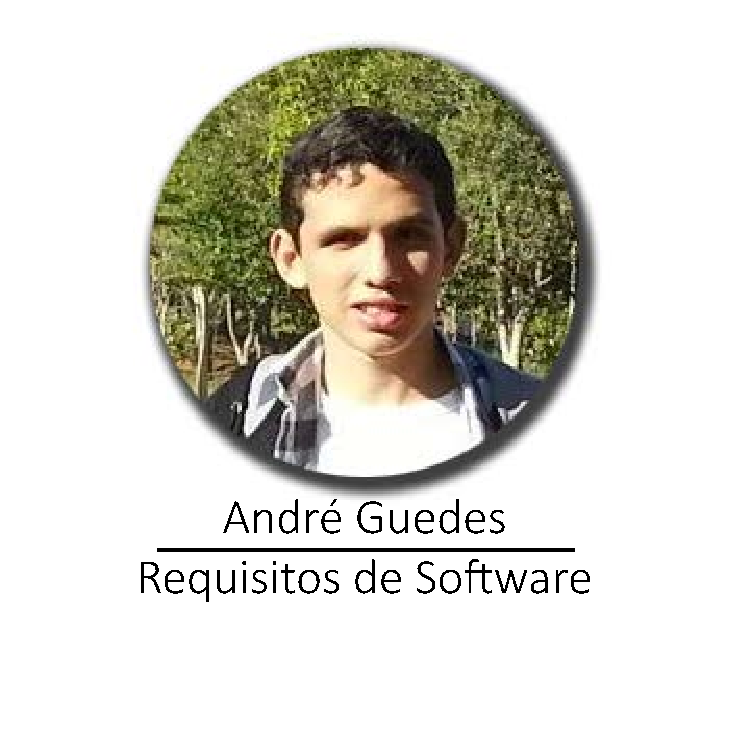
\includegraphics[scale=0.7]{andre_profile}
\end{center}
\ \indent \emph{A interação com um contexto de negócio definido a partir de um processo a ser melhorado trouxe uma experiência distinta a qual achei bastante interessante para o contexto de requisitos de software, pois trouxe uma visão mais clara do limiar entre o contexto de negócio e o contexto da engenharia de requisitos.}
\\ \indent \emph{O contato com o time e os clientes diretamente e constantemente favorece muito as tomadas de decisão e trazem uma perspectiva mais descentralizada onde todos tem uma noção plena do estado atual do projeto, porém também é importante lembrar que esta situação pode levar a equipe a relevar prazos para uma organização mais favorável a sua atual situação.}
\\ \indent \emph{Em suma, o trabalho foi bem encaixado na disciplina e a interação entre as disciplinas foi muito proveitosa, assim como a relação entre os integrantes sempre foi boa, porém trago a sugestão de construção da solução através de um paradigma de programação mais flexível.}
\vspace*{\fill}

\newpage
\vspace*{\fill}
\begin{center}
	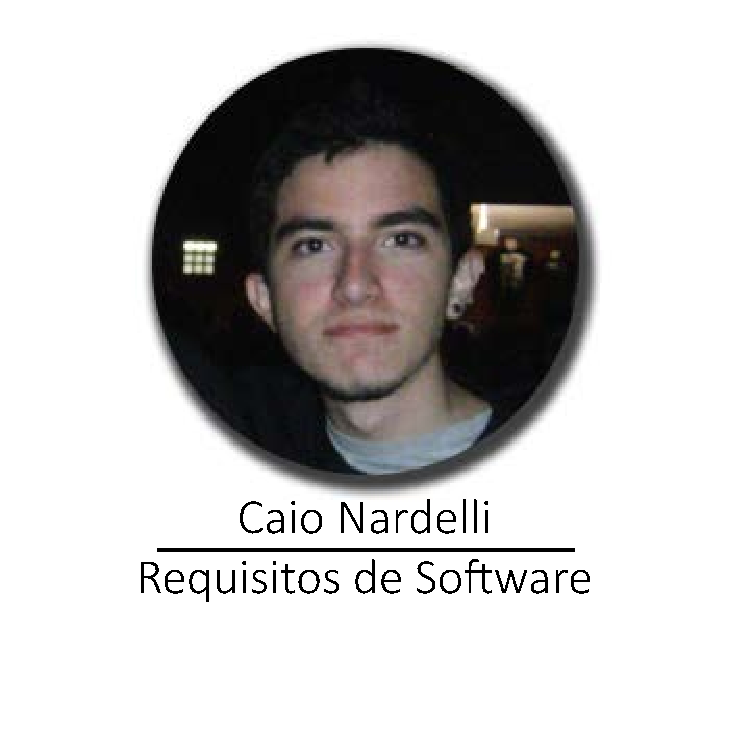
\includegraphics[scale=0.7]{caio_profile}
\end{center}
\ \indent \emph{No contexto desta disciplina de Requisitos de Software, notei que meu crescimento acadêmico foi substancialmente maior ao fazer o trabalho, do que simplesmente estudar teoria para uma prova.}
\\ \indent \emph{Aprendi que a organização e o trabalho em equipe são aspectos fundamentais para o sucesso de um projeto, e que só porque uma ferramenta gera uma solução diretamente pelo processo modelado, não quer dizer que é uma opção melhor.}
\vspace*{\fill}

\newpage
\vspace*{\fill}
\begin{center}
	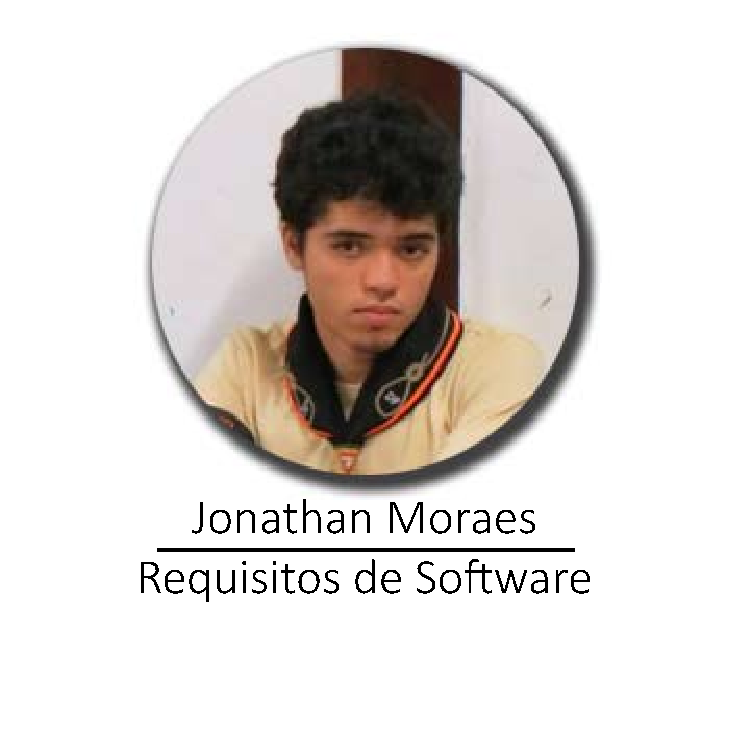
\includegraphics[scale=0.7]{jh_profile}
\end{center}
\vspace*{\fill}
\ \indent \emph{Pude observar com maior afinco as peculiaridades da engenharia de requisitos, onde tornou-se claro para mim a importância de se levantar requisitos com qualidade, gerenciar com eficiência e destreza e interagir com o cliente de forma objetiva e coesa. Ademais, estudar requisitos do ponto de vista do contexto ágil foi uma experiência gratificante, onde busco aplicar nos projetos do meu cotidiano, até mesmo fora do contexto de produção de software.}
\\ \indent \emph{Com o desenvolvimento de um projeto real (mesmo que o contexto seja fictício, todo o desenvolvimento do processo e da execução do mesmo foram feitos buscando o maior teor de profissionalismo possível), aprendi a me adaptar às mudanças, identificar necessidades e otimizar a busca por soluções plausíveis e condizentes com o contexto do negócio.}
\\ \indent \emph{De ponto à considerar, a utilização da ferramenta BPMS foi menos produtiva do que desejei, onde por diversas vezes cogitei o quão mais eficiente seria utilizar uma linguagem de programação para gerar as soluções propostas nos requisitos. Ainda assim, a experiência conquistada ao lidar com uma plataforma totalmente nova e abstrata para mim, buscando com ela uma solução tangível, trouxe uma bagagem didática que até então desconhecia: é preciso sempre se dedicar aos estudos, e em projetos é imprencidível mensurar o esforço que deve ser gasto para adquirir conhecimentos necessários para o desenvolvimento, algo que não conseguimos mensurar com facilidade.}

\newpage
\vspace*{\fill}
\begin{center}
	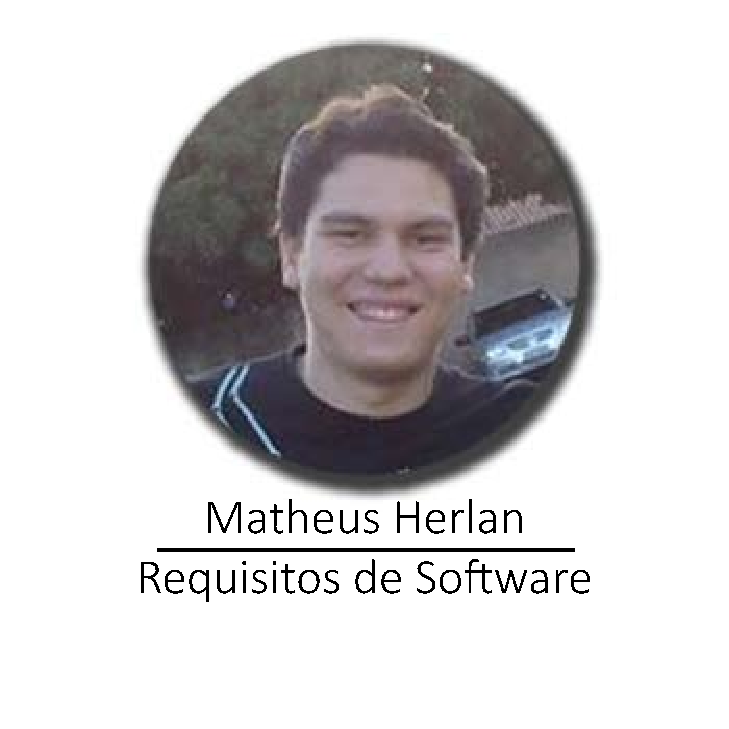
\includegraphics[scale=0.7]{mh_profile}
\end{center}
\ \indent \emph{A realização do trabalho, sem dúvidas, fomentou o conhecimento inerente ao campo de Requisitos de Software. Através dos aspectos teóricos passados em sala de aula e, a partir da apresentação de um contexto de negócio, foi possível correlacionar a teoria à prática, favorecendo ainda mais a assimilação dos conteúdos.}
\\ \indent \emph{No decorrer da realização do trabalho, foi possível constatar que a execução, nem sempre, ocorre conforme o planejado. Inúmeras vezes foram contempladas atualizações no cronograma. Adicionalmente, contatou-se que uma boa solução é obtida a partir de uma análise concisa dos problemas e necessidades.}
\\ \indent \emph{Basicamente, achei interessante a integração entre as disciplinas. Minha única sugestão de melhoria seria no tocante à apresentação da solução. Ao invés de ser BPMS, os alunos poderiam codificar a solução, visto que o Bizagi Studio apresenta muitas limitações (Banco de Dados).}
\vspace*{\fill}

\newpage
\vspace*{\fill}
\begin{center}
	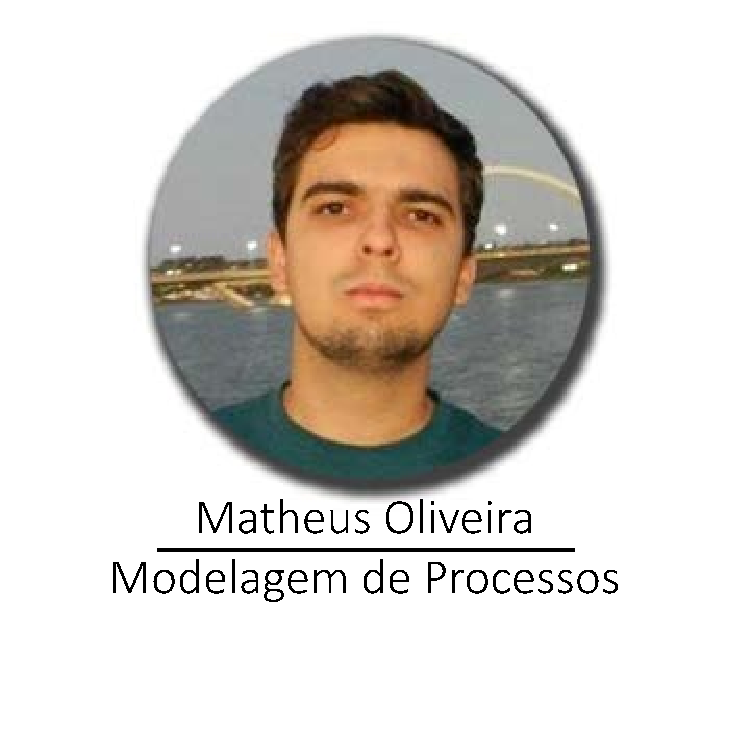
\includegraphics[scale=0.7]{mo_profile}
\end{center}
\ \indent \emph{Como relato de experiência, aprendi muito sobre como modelar um processo de maneira mais sequencial e menos complexa, de modo simplificado.}
\\ \indent \emph{De lições aprendidas: nomenclatura e simbologia na modelagem de processo, priorização de processos, identificação de problemas no processo.}
\\ \indent \emph{Como avaliação geral, acredito que a automação da solução poderia ser feita utilizando uma linguagem de programação convencional.}
\vspace*{\fill}

\newpage
\vspace*{\fill}
\begin{center}
	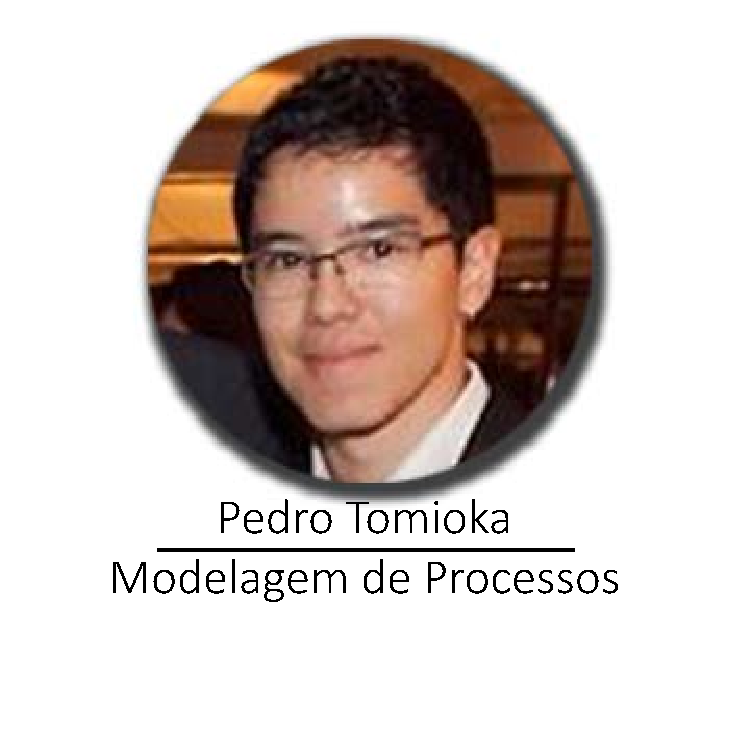
\includegraphics[scale=0.7]{pedro_profile}
\end{center}
\ \indent \emph{Como relato de experiência, aprendi como modelar, simular e propor uma melhoria para um processo de negócio.}
\\ \indent \emph{De lições aprendidas: o estudo do negócio deve ser feito com muito cuidado, considerando todos os stakeholders envolvidos e as restrições impostas por fatores internos e externos}
\\ \indent \emph{Como avaliação geral, as ferramentas de BPMS utilizadas para automação do processo TO-BE são muito confusas e difícil de mexer.}
\vspace*{\fill}


	\section[Considerações do Time]{Considerações do Time}
	\label{sec:feedback_time}
		\input{source/feedback/time}

		\bibliography{bibliografia}
		
	\backmatter
		\bookmarksetup{startatroot} 
		\postextual
    		\printindex

\end{document}
